\documentclass[cic,tc]{infufrgs}
\usepackage[utf8]{inputenc}
\usepackage[T1]{fontenc}
\usepackage{graphicx}
\usepackage{booktabs} 
\usepackage{amsmath} 
%\usepackage{amssymb, amsthm} 
\usepackage{hyperref}
\usepackage{multirow}
\usepackage{array}     
\usepackage{listings}
\usepackage{xcolor}
\usepackage{float}
\usepackage{placeins}

\lstset{
	basicstyle=\ttfamily\small,
	keywordstyle=\color{blue},
	commentstyle=\color{gray},
	stringstyle=\color{orange},
	breaklines=true,
	frame=single,
	captionpos=b
}


\usepackage{tikz}
\usetikzlibrary{arrows,positioning,shapes}


\newcommand{\sat}[1]{\text{Sat}(#1)}
\newcommand{\ex}{\text{EX}}
\newcommand{\eu}{\text{EU}}
\newcommand{\eg}{\text{EG}}
\def\sectionautorefname{Seção}
\def\chapterautorefname{Capítulo}

\title{Lorem Ipsum}
\translatedtitle{Lorem}

\author{Andre Nunes da Silva}{Nicolas} 
\advisor[Prof.~Dr.]{Machado}{Rodrigo} 

\date{Maio}{2026}

\keyword{Verificação Formal, Verificação de Modelos, CTL, Diagramas de Decisão Binária, Rust, NuSMV}
\translatedkeyword{Formal Verification, Model Checking, CTL, Binary Decision Diagrams Rust, NuSMV}

\begin{document}
	
	\maketitle
	
	\begin{abstract}
		A verificação formal de sistemas, especificamente o model checking, desempenha um papel crucial na garantia de corretude de sistemas reativos. Contudo, as abordagens tradicionais frequentemente enfrentam o desafio da explosão de estados. Este trabalho apresenta o desenvolvimento e a análise prática do \texttt{llull-BDD}, um verificador de modelos simbólico implementado em Rust, projetado para avaliar propriedades descritas na lógica temporal Computation Tree Logic (CTL). Para validar a corretude e a eficiência do sistema, foi definido um subconjunto comum da linguagem descritiva SMV, permitindo um benchmark comparativo direto com a ferramenta industrial NuSMV sob diferentes heurísticas de reordenamento de variáveis, como \textit{Sifting} e FORCE. Os resultados experimentais, avaliados por meio de uma análise estatística não-paramétrica multidimensional, revelaram que o \texttt{llull-BDD} é competitivo em problemas mais simples. Por outro lado, o NuSMV demonstrou maior robustez em modelos complexos, adensado devido à sua maturidade comercial. Este projeto demonstra a viabilidade de construir um motor de verificação eficiente em um escopo individual, mapeando as discrepâncias de desempenho em relação ao estado da arte.
	\end{abstract}
	
	\begin{translatedabstract}
		Formal verification of systems, specifically model checking, plays a crucial role in ensuring the correctness of reactive systems. However, traditional approaches frequently face the state explosion problem. This work presents the development and practical analysis of \texttt{llull-BDD}, a symbolic model checker implemented in Rust, designed to evaluate properties described in the temporal logic Computation Tree Logic (CTL). To validate the correctness and efficiency of the system, a common subset of the SMV description language was defined, enabling a direct comparative benchmark against the industrial tool NuSMV under different variable reordering heuristics, such as \textit{Sifting} and FORCE. Experimental results, evaluated through a multidimensional non-parametric statistical analysis, revealed that \texttt{llull-BDD} is competitive in simpler problems. On the other hand, NuSMV demonstrated greater robustness in complex models, which are dense due to its commercial maturity. This project demonstrates the feasibility of building an efficient verification engine within an individual scope, mapping the performance discrepancies relative to the state of the art.
	\end{translatedabstract}
	
	\tableofcontents
	\listoffigures
	\listoftables
	
	\chapter{Introdução}
	
	Este capítulo apresenta a contextualização do trabalho, abordando a relevância da verificação formal, seus objetivos e metodologia.
	
	\section{Motivação}
	
	Segundo \citeonline{clarkeModelChecking2018}, um sistema reativo é um programa cujo comportamento não se resume à mera computação de uma função, isto é, um aparato que simplesmente recebe um \textit{input}, processa-o e retorna um \textit{output}, encerrando-se em um estado de terminação. 
	Um sistema reativo, na verdade, trata-se de um \textit{software} em constante execução e em permanente interação com o seu ambiente, operando em um ciclo contínuo de respostas.
    \citeonline{emerson25mc2008} elenca como exemplos típicos desse tipo de sistema os protocolos de comunicação, os sistemas embarcados e os sistemas operacionais, observando que muitos deles enquadram-se na categoria de missão crítica. 
    Nesses cenários, uma falha de \textit{software} pode causar danos catastróficos, comprometendo tanto a vida humana quanto a estabilidade econômica \cite{emerson25mc2008, baierPrinciplesModelChecking2008a}. 
    Apesar das dificuldades que o desenvolvimento destes sistemas podem apresentar, grande parte deles possui um domínio finito de estados, o que permite uma busca exaustiva por todos os estados alcançáveis pelo sistema \cite{clarkeModelChecking2018}. 
    Dessa forma, torna-se possível verificar, com rigor matemático, se o modelo satisfaz uma determinada propriedade especificada \cite{baierPrinciplesModelChecking2008a}. 
    Na literatura, essa abordagem de exploração exaustiva do espaço de estados é denominada \textbf{verificação de modelos} (\textit{model checking}).
	
	Para isso, o sistema é descrito por meio de um sistema de transição, o qual é verificado com o intuito de determinar se constitui ou não um modelo válido para uma fórmula de lógica temporal \cite{huthLogicComputerScience2000}. 
	Uma lógica temporal é um tipo de lógica modal cujos operadores possuem uma interpretação de tempo, sendo ideal para expressar as propriedades de forma precisa em sistemas reativos que executam por períodos indeterminados \cite{emerson25mc2008}. 
	Especificamente, na verificação de modelos, essas lógicas comumente lidam apenas com operadores direcionados ao tempo futuro. 
	Como a verificação é feita em todo o espaço de estados, o método enfrenta o desafio da \textbf{explosão do espaço de estados}. 
	Essa limitação impulsiona o desenvolvimento de algoritmos voltados à redução do espaço de busca, seja por meio de otimizações diretas em algoritmos explícitos, seja através de abordagens de representação simbólica ou abstrata do modelo \cite{huthLogicComputerScience2000, clarkeModelChecking2018}.
	
	
	Desde a sua gênese, a área de verificação de modelos vem ganhando cada vez mais espaço em aplicações reais. O maior sucesso da área está no contexto de \textit{hardware}, com ferramentas de verificação sendo essenciais em programas de síntese de circuitos digitais \cite{clarkeIntroductionModelChecking2018}. Ao contrário do caso do \textit{hardware}, há uma recepção menor para \textit{softwares}, principalmente em aplicações já desenvolvidas. 
	Contudo, isso é razão para o progresso da verificação de modelos, pois se trata de um campo com problemas ainda a serem resolvidos. 
	Ademais, segundo \citeonline{clarkeIntroductionModelChecking2018}, há três fatos que garantirão o progresso e o sucesso da área, sendo eles: a onipresença de \textit{hardwares} e \textit{softwares} só aumenta, evoluindo ainda mais a complexidade da comunicação e se tornando ainda mais presente em missões críticas; há uma mudança na avaliação de qualidade computacional para além do desempenho e do número de funcionalidades, havendo uma crescente valorização da correção, confiabilidade, segurança e robustez; por fim, os sistemas de transição de estados podem ser usados universalmente como ferramenta em outras áreas, como na produção, \textit{design}, biologia, etc.
	
	
	
	\section{Objetivos e Metodologia}
	Vista a importância da área, o objetivo geral deste trabalho é revisar e analisar de forma prática os principais avanços na verificação de modelos. 
	Dado que existem diferentes lógicas para descrever as propriedades a serem verificadas, o escopo desta investigação será reduzido à lógica \textit{Computation Tree Logic} (CTL) sem \textit{fairness} e sem a construção de contraexemplos. 
	A fundamentação teórica foi estruturada com base nos principais livros-texto da área.
	Além disto, os principais algoritmos foram implementados incrementalmente. Desta forma, foi possível averiguar as dificuldades práticas e teóricas apresentadas. 
	Tudo isto foi feito com o intuito de tentar se aproximar do estado da arte, i.e., o que as principais ferramentas acadêmicas e comerciais consolidadas fazem. 
	
	
	Em virtude disso, o verificador implementado foi comparado diretamente com o NuSMV.
	A comparação serviu para a correção dos algoritmos e também para comparar a eficiência de tempo e memória de uma implementação simples, construída num projeto individual, seguindo como referência o que está disponível em livros-textos, desta forma, contrastando com uma ferramenta industrial aperfeiçoada por décadas.  
	Para efetuar tal comparação, foi definido um subconjunto da linguagem SMV, a linguagem de descrição do modelo usada no NuSMV, para que ambas as ferramentas processem o mesmo modelo.
	
	\subsection{Implementação}
	O verificador implementado neste projeto recebeu o nome de \texttt{llull} para melhor identificação ao longo do texto.
	
	Como o NuSMV é implementado na linguagem C, optou-se por desenvolver o \texttt{llull} também em uma linguagem de programação mais próxima ao hardware, visando assegurar uma comparação de desempenho justa. 
	A linguagem Rust foi escolhida pelo fato de compilar para código nativo sem o intermédio de um \textit{runtime} ou coletores de lixo (garbage collection), assim como C.
	Além disto, apresenta conveniências modernas de desenvolvimento, como o seu gerenciador de pacotes \textit{cargo}, o qual assegura o gerenciamento estrito de dependências e, consequentemente, a reprodutibilidade dos experimentos. 
	Ademais, Rust sobressai-se por ser uma linguagem que oferece garantias nativas de segurança e eficiência no gerenciamento de memória em tempo de compilação.
	
	\subsubsection{Ambiente de Desenvolvimento, Bibliotecas e Reprodutibilidade}
	As bibliotecas e suas versões usadas encontram-se na documentação do projeto nos arquivos \textit{Cargo.toml} e \textit{Cargo.lock}.
	O projeto também foi desenvolvido com o uso do gerenciador de pacotes declarativo \textit{Nix} e sua funcionalidade experimental \textit{flakes}, o que permite a fixação de dependências, permitindo que o projeto tenha uma etapa de compilação (\textit{build}) consistente e reproduzível em diferentes máquinas com os arquivos \textit{flake.nix} e \textit{flake.lock}. Todos os arquivos mencionados estão disponíveis no repositório público do projeto disponível em \cite{??}.
	
	Tanto o desenvolvimento quanto a execução dos experimentos e a coleta de dados foram realizados em um ambiente de hardware com a especificação detalhada na Tabela~\ref{tab:ambiente_hardware}.
	\begin{table}[h!]
		\centering
		\caption{Especificação do Ambiente de Hardware Utilizado nos Testes.}
		\label{tab:ambiente_hardware}
		\begin{tabular}{ll}
			\toprule  
			\textbf{Componente} & \textbf{Especificação Técnica} \\ 
			\midrule  
			Processador (CPU)   & AMD Ryzen 7 5700X (8 núcleos / 16 threads, até 4.6 GHz) \\
			Memória RAM         & 32 GB DDR4 3200 MHz \\
			Armazenamento       & SSD NVMe M.2 (PCIe 4.0, Leitura: 7000 MB/s) \\
			Sistema Operacional & NixOS (Linux Kernel 7.0.10-cachyos-lto / Arquitetura x86\_64) \\ 
			\bottomrule 
		\end{tabular}
		\legend{Fonte: elaborado pelo autor (2026)}
	\end{table}
	
	\subsection{Metodologia dos testes}
	\label{sec:metodologia_t}
	Nesta subseção será apresentada a metodologia de teste usada para comparar os dois verificadores. Serão apresentadas as instâncias, os dados coletados e forma de execução dos programas.
	
	\subsubsection{Instâncias}
	Diversas instâncias foram selecionadas para testar o verificador, ver os limites de cada algoritmo. A preferência foi por problemas paramétricos em que é possível averiguar os efeitos num problema de mesma natureza, mas com um crescimento no número de estados. A forma pela qual cada instância é gerada e quais propriedades são verificadas podem ser vistas na documentação do projeto. Os problemas apresentados são típicos de sistemas reativos: algoritmos de exclusão mútua e protocolos de comunicação, contudo há problemas de outra natureza, como poder ser visto logo abaixo:
	\begin{itemize}
		\item \textit{dining\_N}: o clássico problema do jantar dos filósofos, onde $N$ representa o número de filósofos sentados à mesa.
		\item \textit{counter\_N}: um contador binário de $N$ bits, caracterizado por possuir uma estrutura compacta em algoritmos simbólicos e expansão geométrica em representações explícitas.
		\item \textit{elevator2\_N}: modelo de transição que representa um elevador em um edifício de $N$ andares.
		\item \textit{mcs\_N}: o algoritmo de exclusão mútua em filas de Mellor-Crummey e Scott avaliado para $N$ processos concorrentes.
		\item \textit{sokoban\_N}: modelo de planejamento baseado no jogo Sokoban contendo $N$ blocos de caixas.
		\item \textit{fischer\_N}: o algoritmo de exclusão mútua baseado em tempo de Fischer testado para $N$ processos.
		\item \textit{synapse\_N}: protocolo de coerência de cache Synapse avaliado para $N$ caches independentes.
		\item \textit{train\_gate\_N}: protocolo de controle de tráfego ferroviário (\textit{Train-Gate}) parametrizado para $N$ nós concorrentes.
	\end{itemize}
	
	
	
	As instâncias \textit{elevator2\_N}, \textit{mcs\_N}, \textit{sokoban\_N}, \textit{fischer\_N}, \textit{synapse\_N} e \textit{train\_gate\_N} foram adaptadas a partir dos modelos de referência da suíte BEEM disponíveis em \citeonline{ParaDiSe}. A escolha desse conjunto decorreu da compatibilidade estrutural entre a modelagem em DVE e a linguagem SMV.
	Embora a tradução inicial do formato DVE para SMV tenha sido realizada de forma automatizada com o auxílio de inteligência artificial, todo o processo de mapeamento foi avaliado de forma cruzada. 
	Cada especificação CTL foi verificada manualmente e confrontada entre os ambientes (DiVinE, NuSMV e \texttt{llull}), garantindo que os motores retornassem exatamente o mesmo veredito lógico (verdadeiro ou falso) nos cenários avaliados.
	
	%\subsubsection{Dados coletados}
%	Para cada execução de um modelo SMV, os seguinte dados foram coletados:
%	\begin{itemize}
%		\item \textbf{Tempo de Compilação:} o tempo \textit{parsing} do SMV e construção do BDD ou da estrutura de Kripke explícita.
%		\item \textbf{Tempo de Verificação:} o tempo para verificar todas as propriedades CTL no modelo.
%		\item \textbf{Tempo Total:} o tempo total de execução (compilação+verificação).
%		\item \textbf{Nós Estáticos:} o número de nós do BDD após a compilação.
%		\item \textbf{Nós de Verificação:} o número de nós de BDD após a verificação.
%		\item \textbf{Pico de Memória:} o pico de memória usado durante a execução, coletada com a ferramenta \textit{time} do Linux.
%		\item \textbf{Número de estados:} o número de estados exploráveis pelo algorítimo explícito. 
%	\end{itemize}
	
	
	\subsubsection{Dados Coletados}
	
	Para cada execução de um modelo SMV, foi coletado um conjunto de métricas quantitativas com o objetivo de capturar o comportamento dos verificadores. Coletou-se o \textbf{Tempo de Compilação}, que compreende o \textit{parsing} do arquivo SMV e a construção inicial do BDD ou da estrutura de Kripke explícita, além do \textbf{Tempo de Verificação}, dedicado estritamente à checagem das propriedades CTL. A soma de ambos os componentes estabelece o \textbf{Tempo Total} de execução. 
	
	Também registrou-se o número de \textbf{Nós Estáticos} (gerados logo após a compilação) e de \textbf{Nós de Verificação} (ativos após a conclusão da checagem lógica). Por fim, o \textbf{Pico de Memória} RAM foi monitorado por meio da ferramenta \textit{time} do Linux, enquanto o \textbf{Número de Estados} foi computado para mensurar o espaço explorável pelos algoritmos de abordagem explícita.
	
%	\subsubsection{Execuções}
%	São 30 execuções para cada configuração de instância e heurística de ordenamento de variáveis. 
%	No caso da verificação em BDD, o NUSMV e o llull são executados de forma paralela. 
%	Há um tempo limite estático de 60 segundos para uma execução. 
%	Porém, há também um tempo limite dinâmico, o qual serve para encerrar o processo competidor caso ele demore muito para terminar sua execução, ou seja, assumimos como não sendo competitivo. 
%	Este tempo limite dinâmico é definido pela função $f(t) = t + 10\sqrt{t}+5$ onde $t$ é tempo de execução do primeiro programa (NuSMV ou llull) que terminou, ou seja, caso NuSMV tenha terminado no tempo $t$, llull tem até o tempo $f(t)$ para terminar.
%	Para uma comparação o mais justa possível, o NuSMV foi executado com as seguintes \textit{flags}:
%	\begin{itemize}
%		\item \textbf{\textit{-dxi}}: remove a geração de contra-exemplos, algo que a implementação de llull não faz.
%		\item \textbf{\textit{-coi}}: ativa uma otimização \textit{cone of influence} previa, pois biblioteca de BDDs usada no desenvolvimento deste projeto utiliza algumas otimizações que trazem um efeito similar a esta otimização.
%		\item \textbf{\textit{-mono}}: ativa as relações de transição monolíticas que também é usado em llull.
%	\end{itemize}

\subsubsection{Execuções}

Os experimentos consistiram na realização de 30 execuções independentes para cada configuração de algoritmo, instância e heurística de ordenamento de variáveis. Estabeleceu-se um tempo limite estático de 60 segundos por rodada. 
Há também um tempo limite dinâmico, o qual serve para encerrar o processo competidor caso ele demore muito para terminar sua execução, ou seja, assumimos como não sendo competitivo.
Este tempo limite dinâmico é definido pela função $f(t) = t + 10\sqrt{t}+5$, onde $t$ é tempo de execução do primeiro programa (NuSMV ou llull) que terminou, ou seja, caso NuSMV tenha terminado no tempo $t$, llull tem até o tempo $f(t)$ para terminar.

Com o intuito de garantir condições iguais no a nível de \textit{software}, o NuSMV foi configurado com parâmetros específicos de execução. Utilizou-se a \textit{flag} \texttt{-dxi} para desativar a geração de contraexemplos, funcionalidade ausente no escopo do \texttt{llull}, acompanhada do parâmetro \texttt{-coi} para habilitar a otimização de cone de influência, visto que a biblioteca de BDDs do motor em Rust emprega nativamente reduções semelhantes.
Por fim, ativou-se a opção \texttt{-mono} para forçar o uso de relações de transição monolíticas, sendo esta a arquitetura padrão adotada no desenvolvimento do \texttt{llull}.
	
	
	
	
	\subsubsection{Visualização e teste}
	Foram produzidos gráficos de linha para cada um dos dados coletados. 
	O eixo $y$ dos gráficos representa a métrica medida, enquanto o eixo $x$ é o valor $N$ da instância de um determinado problema. Além destes, na comparação entre heurísticas foram usados os gráficos de sobrevivência de Kaplan-Meier para visualizar o número de instâncias resolvidas ao longo do tempo para cada heurística de ordenamento de variáveis.
	
	Para fundamentar as conclusões das comparações, foram usados os testes estatísticos U de Mann-Whitney e Kolmogorov–Smirnov. 
	O uso do primeiro se dá para avaliar as diferenças locais (em um mesmo $N$) e se justifica pelos seguintes motivos:
	\begin{enumerate}
		\item \textbf{Ausência de Distribuição Normal:} O consumo de recursos computacionais não segue uma distribuição normal, mas sim exponencial.
		
		\item \textbf{Independência das Execuções:} O critério fundamental de independência exigido pelo teste é plenamente satisfeito no nível das execuções (\textit{runs}).
	\end{enumerate}
	O segundo teste, de Kolmogorov-Smirnov, é aplicado de forma global para complementar a análise local, sendo utilizado para avaliar se existe um descolamento estatístico relevante entre as curvas empíricas de desempenho dos programas. Ambos os testes utilizaram um nível de confiança de $95\%$ e foram bicaudais.
	
	
	
	
	\subsection{Uso de Inteligência Artificial Generativa}
	Inteligências artificiais generativas foram usadas no desenvolvimento do verificador. O seu uso principal foi em código não relevante para a compreensão dos algoritmos, como no desenvolvimento do \textit{parsing}, no gerador de instâncias, na produção de testes unitários, na refatoração de código, na interface de linha de comando e na documentação inicial. Os modelos usados foram \textbf{Gemini 3.1} e \textbf{Claude Sonnet 4.6}.
	
	
	
	
	\chapter{Fundamentação Teórica}
	

	Um sistema deve ser descrito seguindo um formalismo específico onde seus componentes e comportamentos principais são abstraídos numa estrutura matemática. O formalismo é a semântica de Kripke apresentada na \autoref{sec:estruturas_de_kripke}. Segundo \citeonline{baierPrinciplesModelChecking2008a}, as propriedades de sistemas reativos são de dois tipos: propriedades de segurança (\textit{safety}) e de vivacidade (\textit{liveness}). Informalmente, as propriedades de segurança garantem que algo de ruim nunca aconteça. Um exemplo mais simples deste tipo é a verificação de invariantes. Já as propriedades de vivacidade garantem que algo de bom aconteça. Qualquer outra propriedade é uma composição de propriedades destes dois tipos. 
	Estas propriedades são formalizadas por meio de lógicas temporais. 
	A \autoref{sec:ctl} apresenta a lógica temporal estudada neste trabalho, incluindo sua interpretação temporal (\autoref{sec:ctl_interpretacao}), sintaxe (\autoref{sec:ctl_sintaxe}) e semântica (\autoref{sec:ctl_semantica}). 
	O formalismo apresentado segue 
	principalmente as construções de \citeonline{blackburnModalLogic2010} para as estruturas de Kripke e \citeonline{baierPrinciplesModelChecking2008a} para CTL.
	
	\section{Estruturas de Kripke}
	\label{sec:estruturas_de_kripke}
	
	A semântica de mundos possíveis (ou semântica de Kripke) é o formalismo padrão para lógicas modais \cite{fittingFirstOrderModalLogic2023}. Um \textit{\textbf{frame}} é um par ordenado $(S, R)$ onde:   
		\begin{itemize}
		\item $S$ é um conjunto finito de \textbf{objetos} (mundos possíveis, estados, etc.).
		\item $R \subseteq S \times S$ é uma \textbf{relação de acessibilidade}.
	\end{itemize}
	\par
	A expressão $(s,s')\in R$ como: $s'$ é acessível a partir do mundo $s$. Um \textit{frame} pode ser facilmente visualizado como um dígrafo. Um \textbf{modelo} $M$ é uma tupla $(F, AP, L)$ em que:
		\begin{itemize}
		\item $F$ é um \textit{frame}.
		\item $AP$ é um conjunto finito de \textbf{proposições atômicas}.
		\item $L: S \to 2^{AP}$ é uma \textbf{função de rotulação} que associa a cada estado um conjunto de proposições que nele são verdadeiras ($M,s\models p\iff p\in L(s)$).
	\end{itemize}
	


	No contexto de verificação de modelos, um sistema reativo é modelado para esta semântica, com o adicional do conjunto $I$ de \textbf{estados iniciais} tal que $I \subseteq S$ para capturar o equivalente de \textbf{sistemas de transição}. Em \citeonline{clarkeHandbookModelChecking2018} e \citeonline{clarkeModelChecking2018}, a tupla $(M,I)$ é chamada de \textbf{estruturas de Kripke}. No caso da \textit{Computation Tree Logic} (CTL), há a restrição adicional de que a relação de acessibilidade $R$ deve ser total, i.e.,  $\forall_s\exists_{s'}((s,s')\in R)$ onde $s,s'\in S$. 
	
	\section{Computation Tree Logic (CTL)}
	\label{sec:ctl}
	As lógicas temporais são usadas como as linguagens de especificação das propriedades \cite{clarkeIntroductionModelChecking2018}.
	Nesta seção, será apresentada a lógica CTL, sua interpretação informal, sintaxe e semântica seguindo a formalização de \citeonline{baierPrinciplesModelChecking2008a}.
	
	\subsection{Interpretação do tempo}
	\label{sec:ctl_interpretacao}
	Uma lógica temporal necessita de uma interpretação específica. 
	Uma interpretação possível é a de tempo linear em que o tempo é visto como uma sequência de acontecimentos únicos, possuindo sempre um possível resultado a cada ponto. 
	Esta interpretação é usada na \textit{Linear Time Logic} (LTL).
	Outra interpretação possível é ver o tempo como uma ramificação de todas possibilidades num determinado ponto. 
	Esta visão permite uma noção de \textbf{caminhos}, os quais alguns podem satisfazer determinada propriedade ou não.
	Dada uma estrutura de Kripke $(M,I)$, a \textbf{árvore de computação}, a estrutura que representa todas os caminhos possíveis, é obtida pelo \textit{unfolding} de $M$ tendo como raiz um estado de $I$ \cite{baierPrinciplesModelChecking2008a}. 
	A lógica de árvore de computação (\textit{Computation Tree Logic}) trabalha com esta interpretação temporal.
	
	\subsection{Sintaxe}
	\label{sec:ctl_sintaxe}
	
	A gramática das fórmulas de CTL sobre um conjunto $AP$ de proposições atômicas é definida através do seguinte conjunto de operadores:
	
	\begin{equation}
		\Phi ::= \top \mid a \mid \neg \Phi \mid \Phi_1 \land \Phi_2 \mid EX \Phi \mid E[\Phi_1 U \Phi_2] \mid EG \Phi
	\end{equation}
	
	Onde $a \in AP$ representa uma proposição atômica. A partir deste conjunto, definimos os demais operadores como abreviações lógicas:
	\begin{equation}
		\begin{aligned}
			AX \Phi &\equiv \neg EX \neg \Phi \\
			EF \Phi &\equiv E[\top U \Phi] \\
			AF \Phi &\equiv \neg EG \neg \Phi \\
			AG \Phi &\equiv \neg EF \neg \Phi \\
			A[\Phi_1 U \Phi_2] &\equiv \neg (E[\neg \Phi_2 U (\neg \Phi_1 \land \neg \Phi_2)] \lor EG \neg \Phi_2)
		\end{aligned}
		\label{eq:equiv}
	\end{equation}


	\subsection{Semântica}
	\label{sec:ctl_semantica}
	Seja $a$ uma proposição atômica de $AP$, $\Phi$ uma fórmula CTL, um \textit{frame} $F = (S,R)$ e um modelo $M = (F, AP, L)$. Definimos um caminho como uma tupla infinita de estados $(s_0,s_1,s_2,...)$. A satisfação ($\models$) de uma fórmula num estado $s_0\in S$ do modelo $M$ é definida da seguinte forma:
	\begin{itemize}
		\item $M, s_0 \models a \iff a \in L(s_0)$
		\item $M, s_0 \models \neg \Phi \iff M, s_0 \not\models \Phi$
		\item $M, s_0 \models \Phi_1 \land \Phi_2 \iff M, s_0 \models \Phi_1 \text{ e } M, s_0 \models \Phi_2$
		\item $M, s_0 \models EX \Phi \iff \exists \pi = (s_0, s_1, \dots) \text{ tal que } M, s_1 \models \Phi$
		\item $M, s_0 \models EG \Phi \iff \exists \pi = (s_0, s_1, \dots) \text{ tal que } \forall i \geq 0, M, s_i \models \Phi$
		\item $M, s_0 \models E[\Phi_1 U \Phi_2] \iff \exists \pi = (s_0, s_1, \dots) \text{ tal que } \exists j \geq 0 \mid (M, s_j \models \Phi_2 \land \forall k < j, M, s_k \models \Phi_1)$
	\end{itemize}
	As abreviações \eqref{eq:equiv} podem ser definidas independentemente, para melhor compreensão destas, da seguinte forma:
	\begin{itemize}
		\item  $M, s_0 \models AX \Phi \iff \forall \pi = (s_0, s_1, \dots) \text{ tal que } M, s_1 \models \Phi$
		\item  $M, s_0 \models EF \Phi \iff \exists \pi = (s_0, s_1, \dots), \exists i \ge 0 \text{ tal que } M, s_i \models \Phi$
		\item  $M, s_0 \models AF \Phi \iff \forall \pi = (s_0, s_1, \dots), \exists i \ge 0 \text{ tal que } M, s_i \models \Phi$
		\item  $M, s_0 \models AG \Phi \iff \forall \pi = (s_0, s_1, \dots) \text{ tal que } \forall i \ge 0, M, s_i \models \Phi$
		\item  $M, s_0 \models A[\Phi_1 U \Phi_2] \iff \forall \pi, \exists j \ge 0 \text{ tal que } (M, s_j \models \Phi_2 \land \forall k < j, M, s_k \models \Phi_1)$
	\end{itemize}
	
	%
%	\subsubsection{Compreensão informal dos operadores temporais}
%	\label{sec:ctl_informal}
%	Cada operador temporal pode ser lido informalmente assim:
%	\begin{itemize}
%		\item \textbf{$EX\phi$:} $\Phi$ é satisfeita no próximo estado de algum caminho.
%		\item \textbf{$AX\phi$:} $\Phi$ é satisfeita no próximo estado de todos caminhos possíveis.
%		\item \textbf{$EG\phi$:} $\Phi$ é satisfeita no em todos estados de algum caminho.
%		\item \textbf{$AG\phi$:} $\Phi$ é satisfeita no em todos estados de todos caminho possíveis.
%		\item \textbf{$EF\phi$:} $\Phi$ é eventualmente satisfeita em algum estado de algum caminho.
%		\item \textbf{$AF\phi$:} $\Phi$ é eventualmente satisfeita em algum estado de todos caminhos possíveis.
%		\item \textbf{$E[\Phi_1 U \Phi_2]$:} $\Phi_1$ é satisfeita até que $\Phi_2$ é satisfeita em algum caminho.
%		\item \textbf{$A[\Phi_1 U \Phi_2]$:} $\Phi_1$ é satisfeita até que $\Phi_2$ é satisfeita em todos os caminhos possíveis.
%	\end{itemize}
	
	
	\chapter{SMV, NuSMV e SSMV}
	A escolha por realizar a comparação com o NuSMV se dá pelo fato de o SMV ser pioneiro na verificação simbólica de modelos. 
	Além disso, o SMV foi concebido inicialmente para a lógica CTL, sendo então facilmente conversível para as representações simbólicas desta lógica, a qual define o escopo deste trabalho.
	
	
	Mais especificamente, este trabalho realiza a comparação com a reimplementação NuSMV. 
	Há razões de interesse prático para esta escolha: 
	Em primeiro lugar, possui código aberto, permitindo uma análise mais minuciosa das diferenças com a implementação de \texttt{llull}. 
	Em segundo lugar, o NuSMV atualmente ainda é relevante. 
	Por exemplo, o SMV é a linguagem de descrição (modelagem) e o NuSMV é um dos núcleos do nuXmv, o qual obteve destaque recente em uma competição de verificação de modelos em hardware \cite{HWMCC25} e apresenta uso industrial relevante para um design da NASA \cite{rozierMoXIIntermediateLanguage2025}.
	
	Para evitar trabalho desnecessário aos propósitos desta pesquisa, reduzimos a linguagem SMV no verificador \texttt{llull} para um subconjunto (SSMV, de \textit{Subset} SMV) contendo apenas as estruturas de dados primitivas (inteiros, enumerações e boolianos) e um único módulo (\texttt{MAIN}), sem especificações LTL e sem diretivas específicas de \texttt{FAIRNESS} e \texttt{TRANSITION}.
	A gramática SSMV foi construída de forma mais restrita visando à simplicidade de implementação, o que leva à sua não classificação estrita como um subconjunto da linguagem SMV. Entretanto, as instâncias foram construídas de modo que ambos os verificadores consigam compreender e reproduzir os mesmos resultados na avaliação da especificação.
		
	
	
	
\chapter{Verificação de modelos explícita}

Neste capítulo, será apresentada a verificação de modelos explícita, na qual o modelo SMV é representado em uma estrutura de Kripke. Os resultados obtidos com esta abordagem serão retomados na comparação com os motores simbólicos, apresentada no Capítulo~\ref{ch:ver_simbolica}.


\section{Algoritmo de rotulação (\textit{labelling})}
O algoritmo para verificação explícita implementado foi o algoritmo de rotulação, apresentado primeiramente no trabalho seminal de \citeonline{clarkeDesignSynthesisSynchronization1982}. 
A formulação usada como referência inicial foi a de \citeonline{huthLogicComputerScience2000}. 
Em linhas gerais, o procedimento opera de maneira \textit{bottom-up} sobre a árvore de sintaxe abstrata (AST) da fórmula CTL alvo. 
O algoritmo decompõe a especificação em todas as suas subfórmulas. 
A partir disso, realiza-se uma varredura exaustiva que avalia cada subfórmula contra todos os estados da estrutura de Kripke. 
À medida que um estado satisfaz determinado operador, ele é rotulado com a respectiva subfórmula, progredindo recursivamente até que a fórmula principal seja avaliada.
A implementação em Rust pode ser acessada no código-fonte disponível em \citeonline{??}.

\section{Notas de Implementação}
Para evitar ao máximo o desperdício de memória desse algoritmo, algumas escolhas cruciais de estruturas de dados foram feitas seguindo o paradigma \textit{Data-Oriented Design} (DOD). 
O confronto entre o protótipo inicial ingênuo e o motor refatorado sob as premissas do DOD mostrou uma redução de aproximadamente 70\% no pico de consumo de memória em execuções de teste isoladas, justificando a adoção das técnicas descritas a seguir.

Uso de arenas, que são vetores unidimensionais, para armazenar os dados. Qualquer referência aos dados é feita por um identificador único, o qual representa a posição da arena na qual ele se encontra. Com essa estrutura de dados, é possível implementar um mecanismo para evitar a duplicação de dados. Por exemplo, uma mesma proposição não precisa ser alocada mais de uma vez na memória, mesmo que apareça repetidamente na descrição ou na especificação.

O \textit{frame} de transições é representado por uma matriz CSR (\textit{Compressed Sparse Row}), ideal para grafos esparsos e exploração de localidade na memória.
Os conjuntos de estados são representados internamente por \textit{bitsets}, permitindo que as operações de conjuntos sejam executadas bit a bit (\textit{bitwise}).
Por fim, no processo de compilação, o modelo em SSMV é transformado numa árvore de sintaxe abstrata (AST), que então é transformada numa representação intermediária mais simples para a etapa de codificação para uma estrutura de Kripke. Além disso, há uma estrutura de Kripke no formato de um grafo convencional que então é transformado na representação de matriz CSR.
   

\section{O problema da explosão de estados}

O principal problema da verificação explícita, em especial do algoritmo de rotulagem, é sofrer, com mais força, do maior desafio da verificação de modelos: a explosão de estados. 
Isso pode ser exemplificado de forma simples: seja um modelo $M$ com $N$ variáveis boolianas; assumindo que todas as combinações de valores sejam acessíveis, teremos ao final $2^N$ estados possíveis.
Assim, o obstáculo do algoritmo de rotulação surge principalmente no tamanho do modelo, dada sua complexidade polinomial $\mathcal{O}(\lvert M \rvert \cdot \lvert f \rvert)$, onde $\lvert M \rvert$ é o tamanho do modelo (a soma do número de estados e do número de transições) e $\lvert f \rvert$ é o tamanho da fórmula \cite{baierPrinciplesModelChecking2008a}.
O esforço central dos pesquisadores, então, consiste em encontrar formas de reduzir o tamanho da representação do espaço de estados, construindo representações simbólicas ou abstratas \cite{clarkeIntroductionModelChecking2018}.



	
	\chapter{Diagramas de decisão binário (Binary Decision Diagrams)}
	
	Neste capítulo, será apresentada a principal estrutura de dados usada para a representação simbólica da lógica CTL. 
	Em linhas gerais, utiliza-se um \textit{Binary Decision Diagram} (BDD) para representar de forma compacta uma \textit{switching function}, a qual expressa um conjunto de estados que satisfazem uma fórmula. 
	Toda a apresentação deste modelo serve como base teórica para a compreensão dos resultados. O conteúdo deste capítulo segue o que foi apresentado em \citeonline{baierPrinciplesModelChecking2008a}.
	
	\section{Switching Functions}
	
	Seja um conjunto de variáveis boolianas $Var = \{x_1,x_2,x_3,...,x_n\}$. 
	Uma \textbf{avaliação} é uma atribuição de valores boolianos ($0$ ou $1$) a essas variáveis; ou seja, uma avaliação é uma função $\eta: Var \to \{0,1\}$. 
	O termo $Eval(Var)$ denota o conjunto de \textbf{todas as avaliações possíveis sobre o conjunto de variáveis} \cite{baierPrinciplesModelChecking2008a}.
	
	No contexto de verificação de modelos, cada estado é definido por um conjunto de variáveis boolianas com uma valoração específica para cada uma delas; por exemplo, um estado $s$ poderia ser representado por $\{x_1=1, x_2=0\}$. 
	Uma \textbf{\textit{switching function}} é uma função $f: Eval(Var) \mapsto \{0,1\}$, a qual é utilizada para representar um conjunto de satisfação, isto é, o conjunto de estados nos quais uma fórmula é satisfazível \cite{baierPrinciplesModelChecking2008a}. 
	Por exemplo, utiliza-se a \textbf{função característica} $\chi_T$ para representar um subconjunto de estados $T \subseteq S$:
	
	\begin{equation}
		\chi_T(s) = 1 \iff s \in T
	\end{equation}
	
	Dessa forma, operações sobre conjuntos (união, interseção, complemento, etc.) são realizadas por meio de operações lógicas ($\lor$, $\land$, $\neg$, etc.) sobre as \textit{switching functions}. 
	
	
	
	\section{Diagramas de decisão binário (Binary Decision Diagrams)}
	
	Um BDD é uma estrutura de dados usada para representar uma \textit{switching function}. Seja o conjunto de variáveis $Var =\{x_1,x_2,...,x_n\}$. Um \textit{Binary Decision Diagram} é uma tupla $(V,V_I,V_T,succ_0,succ_1,var,val,v_0)$ \cite{baierPrinciplesModelChecking2008a}. Cada elemento da tupla é definido como:
	\begin{itemize}
		\item Um conjunto finito de nós $V$.
		\item Os conjuntos $V_I\subset V$ e $V_T\subset V$, tais que $V_I$ são os nós internos, $V_T$ são os nós terminais e $V_I\cap V_T=\emptyset$.
		\item As funções de sucessores $succ_0: V_I\to V$ e $succ_1: V_I\to V$.
		\item A função de atribuição de nós internos a variáveis $var: V_I\to Var$.
		\item A função de atribuição de valores boolianos a nós terminais $val: V_T\to \{0,1\}$.
		\item Um nó raiz $v_0$, no qual $\neg\exists x(succ_1(x)=v_0\lor succ_0(x)=v_0)$.
	\end{itemize}
	
	Graficamente, um BDD representa o processo de tomada de decisão em que cada nó interno corresponde a uma variável booliana avaliada, estendendo o conceito de uma Árvore de Decisão Binária por meio do compartilhamento de subgrafos isomórficos.
	Em geral, um BDD é um grafo direcionado que pode assumir diversas configurações.
	
	Segundo \citeonline{baierPrinciplesModelChecking2008a}, em aplicações de verificação de modelos, trabalha-se com diagramas mais comportados, sendo as principais propriedades deles definidas da seguinte forma:
	
	\begin{itemize}
		\item \textbf{Ordered Binary Decision Diagram (OBDD)}: Um $\mathcal{P}$-OBDD é um BDD $\mathcal{B}$ que respeita um ordenamento de variáveis $(x_1,x_2,...,x_n)$, no qual $x_i<x_{i+1}$ para qualquer valor de $i\in{\{1,...,n\}}$. A função de sucessores deve ser consistente com a relação de ordem; ou seja, se $succ(v_i) = v_j$, então $var(v_i)<var(v_j)$.
		\item \textbf{Reduced Ordered Binary Decision Diagram (ROBDD)}: Um ROBDD é um $\mathcal{P}$-OBDD no qual $\forall v,w\in V(v\neq w\to f_v \neq f_w)$, em que $f_v$ é a função induzida de um BDD tomando o nó $v$ como raiz. Um ROBDD é uma representação canônica e única de qualquer função booliana numa ordem de variáveis. Isso possui duas vantagens: a primeira é que todo OBDD pode ser reduzido por meio de regras de redução, economizando memória; a segunda é a possibilidade verificar a equivalência da função em tempo constante, simplesmente verificando se as funções compartilham o mesmo nó raiz.
		\item \textbf{Shared Ordered Binary Decision Diagram (SOBDD)}: Cada função possui um ROBDD para ser representada; porém, manter diversos ROBDDs pode ser custoso, pois há redundâncias e duplicação de funções. Para evitar isso, utiliza-se o SOBDD, um OBDD com diversas raízes (um conjunto de raízes em vez de um único $v_0$). Cada função é representada por uma raiz, e as diferentes funções compartilham nós de funções isomórficas. Bibliotecas de BDD implementam esse tipo para reduzir o uso de memória.
	\end{itemize}  
	
	
	\subsection{Exemplo: Shared OBDD (SOBDD)}
	Neste exemplo, as funções $f = x \land y$ e $g = z \lor (x \land y)$ são representadas simultaneamente. A subexpressão $(x \land y)$ é calculada e armazenada apenas uma vez, sendo compartilhada por ambas as raízes.
	
	\begin{center}
		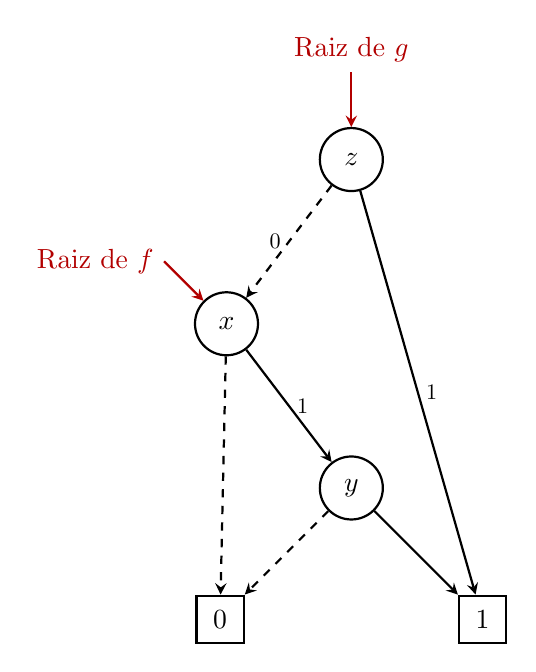
\begin{tikzpicture}[
			node distance=1.5cm and 2cm,
			v/.style={circle, draw, minimum size=8mm, thick},
			t/.style={rectangle, draw, minimum size=6mm, thick},
			root/.style={draw, stealth-, thick, red!70!black},
			>=stealth,
			thick
			]
			
			% Nós da estrutura
			\node[v] (z) {$z$};
			\node[v] (x) [below left=of z, xshift=1cm] {$x$};
			\node[v] (y) [below right=of x, xshift=-1cm] {$y$};
			
			% Terminais únicos
			\node[t] (t0) [below left=1.5cm of y] {0};
			\node[t] (t1) [below right=1.5cm of y] {1};
			
			% Definição das Raízes (Entry Points)
			\draw[root] (z.north) -- ++(0,0.7) node[above] {Raiz de $g$};
			\draw[root] (x.north west) -- ++(-0.5,0.5) node[left] {Raiz de $f$};
			
			% Arestas de Z (Função g)
			\draw[->] (z) -- (t1) node[midway, right, scale=0.8] {1}; % Se z=1, g=1
			\draw[->, dashed] (z) -- (x) node[midway, left, scale=0.8] {0}; % Se z=0, g depende de (x and y)
			
			% Arestas de X (Compartilhadas por f e g)
			\draw[->] (x) -- (y) node[midway, right, scale=0.8] {1};
			\draw[->, dashed] (x) -- (t0);
			
			% Arestas de Y (Compartilhadas)
			\draw[->] (y) -- (t1);
			\draw[->, dashed] (y) -- (t0);
			
		\end{tikzpicture}
	\end{center}
	
	
	
	
	\chapter{Codificação de Modelos SSMV para \textit{switching functions}}
	\label{ch:code}
	
	Em \citeonline{baierPrinciplesModelChecking2008a}, apresenta-se como codificar estruturas de Kripke (sistemas de transição, na terminologia dos autores) em \textit{switching functions}. 
	Como se utiliza um modelo baseado em SMV, é necessário realizar um tratamento específico para cada tipo de dado e expressão da linguagem de descrição, tais como atribuições, condicionais, enumerações, etc.
	Nos materiais consultados, não foi encontrada a formalização dessa codificação.
	Assim, este trabalho propõe o desenvolvimento de uma codificação própria para a linguagem de descrição, a qual é detalhada no presente capítulo.  
	
	
	\section{Codificação de Variáveis}
	Variáveis de domínios finitos são mapeadas para vetores de bits boolianos de acordo com o tamanho do domínio do tipo de dado. 
	Seja $|dom(x)|$ a cardinalidade do domínio de uma variável do SSMV (sejam naturais, booleanas ou enumerações). 
	A quantidade de variáveis boolianas do BDD necessárias para representar cada variável do SSMV é dada por $\lceil \log_2(|dom(x)|)\rceil$. Para cada variável booliana criada, é obrigatório gerar um número idêntico de variáveis boolianas futuras, as quais são usadas para representar as expressões \textit{next} (ou seja, como o valor de uma variável é atualizado).
	
	Por exemplo, caso $n: 0..7$ seja uma variável do tipo natural, teremos $|dom(n)| = 8$, logo $\lceil \log_2(8)\rceil = 3$. Ou seja, serão necessárias três variáveis lógicas (por exemplo, $x_1$, $x_2$ e $x_3$) para codificar a variável $n$ do SSMV. Adicionalmente, serão requeridas as variáveis de estado futuro correspondentes: $x_1'$, $x_2'$ e $x_3'$.
	
	\section{Codificação de expressões boolianas}
	A partir desta seção, será usado $f_\phi$ para simbolizar a \textit{switching function} que representa a expressão $\phi$ da linguagem de descrição SSMV, sendo $\phi$ uma expressão arbitrária.
	Primeiramente, para cada expressão booliana, basta codificar as subexpressões para sua respectiva \textit{switching function} e realizar a operação booliana:
	\begin{itemize}
		\item \textbf{a \& b}: $f_{\text{a\&b}} = f_a\land f_b$.
		\item \textbf{a | b}: $f_{\text{a|b}} = f_a\lor f_b$.
		\item \textbf{!a}: $f_{\text{!a}} = \neg f_a$.
		\item \textbf{a->b}: $f_{\text{a->b}} = f_a\to f_b$.
	\end{itemize}
	

	
	\section{Codificação de Expressões Relacionais}
	Sejam $\textbf{a}$ e $\textbf{b}$ dois vetores de bits boolianos de largura $n$ (normalizados via extensão de zeros caso possuam tamanhos originais distintos), onde $x_i$ representa os bits que codificam $\textbf{a}$ e $y_i$ os bits que codificam $\textbf{b}$, indexados do bit menos significativo ($i=1$) ao mais significativo ($i=n$).
	\begin{itemize}
		\item \textbf{a = b}: $f_{\text{a=b}} = \bigwedge_{i=1}^n (x_i \leftrightarrow y_i)$
		\item \textbf{a != b}: $f_{\text{a!=b}} = \neg f_{\text{a=b}}$
		\item \textbf{a > b}: $f_{\text{a>b}} = \bigvee_{i=1}^n \left( (x_i \land \neg y_i) \land \bigwedge_{j=i+1}^n (x_j \leftrightarrow y_j) \right)$
		\item \textbf{a <= b}: $f_{\text{a<=b}} = \neg f_{\text{a>b}}$
		\item \textbf{a < b}: $f_{\text{a<b}} = f_{\text{b>a}}$
		\item \textbf{a >= b}: $f_{\text{a>=b}} = \neg f_{\text{a<b}}$
	\end{itemize}
	
	
	\section{Codificação de Operações Aritméticas}
	A aritmética de vetores de bits é implementada simulando circuitos combinatórios através de operações lógicas. 
	
	\subsection*{Adição (Ripple Carry Adder)}
	A soma de dois vetores de bits $\textbf{a}$ e $\textbf{b}$ de tamanho $n$ é realizada bit a bit, propagando um bit de transporte (\textit{carry}). O bit de transporte inicial é definido como $c_0 = 0$. Para cada bit $i \in \{1, \dots, n\}$, o bit de soma $s_i$ e o próximo \textit{carry} $c_{i}$ são calculados como:
	\begin{itemize}
		\item $s_i = x_i \oplus y_i \oplus c_{i-1}$
		\item $c_i = (x_i \land y_i) \lor ((x_i \oplus y_i) \land c_{i-1})$
	\end{itemize}
	
	\subsection*{Subtração (Complemento de Dois)}
	A subtração $\textbf{a} - \textbf{b}$ é convertida em uma operação de soma utilizando a representação de complemento de dois. Matematicamente, a operação é equivalente a $\textbf{a} + \neg \textbf{b} + 1$. 
	\begin{itemize}
		\item O \textit{carry} inicial é definido como $c_0 = 1$, representando o $+1$ da fórmula.
		\item $sub_i = x_i \oplus \neg y_i \oplus c_{i-1}$.
	\end{itemize}
	
	  \section{Relações de Atribuição}
	\subsection*{Enumerações e Conjuntos}
	Seja um conjunto de elementos determinísticos $\{e_1, e_2, \dots, e_k\}$, a função que atribui uma constante não-determinística a uma variável de estado futuro $x'$ é expressa pela disjunção das relações individuais de equivalência:
	\begin{equation}
		f_{enum} = \bigvee_{i=1}^k (x' \leftrightarrow e_i)
	\end{equation}
	
	\subsection*{Condicionais (\textit{Case})}
	As expressões condicionais avaliam uma sequência de cláusulas de guarda $\{c_1, c_2, \dots, c_n\}$ associadas a seus respectivos blocos de atribuição final $\{r_1, r_2, \dots, r_n\}$. No modelo SSMV, essas estruturas mapeiam o comportamento lógico do operador \textit{next}, assumindo a forma \textit{next(x) := case c\_1 : r\_1; \dots; esac;}.
	
	A compilação é realizada por meio do encadeamento ordenado de operadores \textit{if-then-else} ($ITE$), processados recursivamente a partir da última cláusula:
	\begin{equation}
		f_{case} = ITE(c_1, f_{x'=r_1}, ITE(c_2, f_{x'=r_2}, \dots ITE(c_n, f_{x'=r_n}, \text{false}) \dots ))
	\end{equation}
	
	\section{Relação de Transição Transicional (\texorpdfstring{$\Delta$}{Delta})}
	A relação de transição global do sistema é codificada como uma fórmula booliana monolítica que restringe o comportamento conjunto de todas as variáveis do presente ($s$) e suas respectivas projeções no estado futuro ($s'$):
	\begin{equation}
		\Delta(s, s') = \bigwedge_{v \in Var} \mathcal{R}_v(s, s')
	\end{equation}
	
	Onde $\mathcal{R}_v(s,s')$ representa a relação de atribuição construída para a variável $v$ com base no bloco gramatical do modelo SSMV, integrando as seguintes regras de mapeamento:
	\begin{itemize}
		\item \textbf{Atribuição Simples:} $\mathcal{R}_v = (x' \leftrightarrow f_x(s))$
		\item \textbf{Conjuntos/enumerações:} $\mathcal{R}_v = \bigvee_{i=1}^k(x' \leftrightarrow e_i)$
		\item \textbf{Condicionais (Case):} $\mathcal{R}_v = ITE(c_1, \mathcal{R}_{x_1}, ITE(c_2, \mathcal{R}_{x_2}, \dots, \text{false}))$
	\end{itemize}
	
	
	
	
	\chapter{Verificação de Modelos Simbólica}
	\label{ch:ver_simbolica}
	
	Neste capítulo, serão apresentadas algumas informações sobre o algoritmo implementado, além de uma comparação entre o lull e o NuSMV. 
	Na subseção final, essa mesma análise será realizada, mas com a adição de heurísticas de reordenamento de variáveis e a avaliação de seu impacto na verificação.
	
	\section{Algoritmo e Notas de Implementação}
	A representação de \textit{switching functions} por BDDs foi realizada utilizando-se a biblioteca 
	\textbf{OxiDD}, apresentada em \citeonline{husungOxiDDSafeConcurrent2024}.
	A codificação foi desenvolvida seguindo as definições do Capítulo~\ref{ch:code}. 
	O algoritmo implementado segue a exata mesma estrutura do algoritmo explícito, com a óbvia diferença de utilizar BDDs como estruturas de dados e operar diretamente sobre eles. Com base em algumas recomendações de \citeonline{baierPrinciplesModelChecking2008a}, algumas informações mais específicas sobre a implementação são detalhadas a seguir:
	\begin{itemize}
		\item As variáveis $x_i$ e as variáveis futuras $x_i'$ são sempre intercaladas na ordem $(x_1,x_1', x_2,x_2', \dots, x_n,x_n')$.
		Essa configuração demonstra-se experimentalmente mais eficiente para as operações em BDDs. 
		\item Utilizou-se a operação \textit{and-exists} no processamento dos operadores temporais, visto que ela está nativamente disponível na biblioteca OxiDD.
		\item Fora das recomendações, para as operações aritimética em BDDs, para que os números tivessem o mesmo tamanho, eles foram expandidos (\textit{padding}) para 32 bits. 
		\item No processo de compilação, o modelo em SSMV é transformado numa AST, que então é transformado numa representação intermediária mais simples para a etapa de codificação para BDD.
	\end{itemize}
	
	\section{Resultados e Avaliação}
	\label{sec:resultados_avaliacao}
	
	A definição de quais dados foram coletados, a forma como as comparações foram feitas, os testes estatísticos utilizados e a maneira como as informações são dispostas foram estabelecidos na seção de metodologia (\ref{sec:metodologia_t}). Assim, o presente tópico delimita-se à apresentação dos resultados e à respectiva avaliação deles. Será apresentada uma subseção por instância caso os resultados da variação escalar sejam relevantes. A razão para não dedicar a cada modelo uma subseção isolada será detalhada na Seção~\ref{sec:outras_inst}.
	
	% =========================================================================
	% 1. DINING
	% =========================================================================
	\subsection{Problema dos Filósofos (\textit{Dining})}
	\label{sec:res_dining}
	
	O problema clássico do jantar dos filósofos foi avaliado sob a configuração de ordenamento padrão (\textit{default}). O parâmetro de escala $N$ representa o número de filósofos concorrentes sentados à mesa, expandindo-se de $N=2$ até $N=16$.
	
	% =========================================================================
	% BLOCO UNIFICADO: GRÁFICOS E TABELA NO MESMO AMBIENTE FLUTUANTE
	% =========================================================================
	\begin{figure}[htbp]
		\centering
		% Linha 1: Tempos
		\begin{minipage}{0.32\textwidth}
			\centering
			\includegraphics[width=\textwidth]{figures/resultados_dining/grafico_log_total_ms_dining_default.pdf}
			\caption{Tempo Total.}
			\label{fig:dining_total_default}
		\end{minipage}
		\hfill
		\begin{minipage}{0.32\textwidth}
			\centering
			\includegraphics[width=\textwidth]{figures/resultados_dining/grafico_log_verify_ms_dining_default.pdf}
			\caption{Tempo de Verificação.}
			\label{fig:dining_verify_default}
		\end{minipage}
		\hfill
		\begin{minipage}{0.32\textwidth}
			\centering
			\includegraphics[width=\textwidth]{figures/resultados_dining/grafico_log_compile_ms_dining_default.pdf}
			\caption{Tempo de Compilação.}
			\label{fig:dining_compile_default}
		\end{minipage}
		
		\vspace{0.8em}
		
		% Linha 2: Recursos
		\begin{minipage}{0.48\textwidth}
			\centering
			\includegraphics[width=\textwidth]{figures/resultados_dining/grafico_log_peak_mem_mb_dining_default.pdf}
			\caption{Pico de Memória RAM (MB).}
			\label{fig:dining_mem_default}
		\end{minipage}
		\hfill
		\begin{minipage}{0.48\textwidth}
			\centering
			\includegraphics[width=\textwidth]{figures/resultados_dining/grafico_log_verification_nodes_dining_default.pdf}
			\caption{Quantidade de Nós no BDD.}
			\label{fig:dining_nodes_default}
		\end{minipage}
		
		\vspace{1.5em} % Espaçamento regulatório entre as figuras e a tabela
		
		% Linha 3: Tabela Estatística Embutida
		% Usamos o comando \captionof{table}{...} para manter a legenda correta de Tabela
		% mesmo estando dentro de um ambiente "figure".
		\captionof{table}{Resultados do teste de Mann-Whitney U e Kolmogorov-Smirnov (KS) para a instância \textit{dining} entre llull-BDD e NuSMV-static.}
		\label{tab:estatistica_dining_default}
		\small % Reduz ligeiramente a fonte para garantir que o bloco cabe perfeitamente na página
		\begin{tabular}{rccccc}
			\toprule
			\textbf{N} & \textbf{Tempo Total} & \textbf{Compilação} & \textbf{Verificação} & \textbf{Memória} & \textbf{Nós BDD} \\
			\midrule
			2  & Empate      & Empate       & Empate      & NuSMV       & \textbf{llull} \\
			4  & \textbf{llull} & NuSMV       & \textbf{llull} & NuSMV       & \textbf{llull} \\
			6  & \textbf{llull} & NuSMV       & \textbf{llull} & NuSMV       & \textbf{llull} \\
			8  & \textbf{llull} & NuSMV       & \textbf{llull} & NuSMV       & \textbf{llull} \\
			10 & \textbf{llull} & NuSMV       & \textbf{llull} & NuSMV       & \textbf{llull} \\
			12 & \textbf{llull} & NuSMV       & \textbf{llull} & \textbf{llull} & \textbf{llull} \\
			14 & \textbf{llull} & NuSMV       & \textbf{llull} & NuSMV       & NuSMV \\
			\midrule
			\textbf{KS} & Equivalente & Divergente & Equivalente & Divergente & Divergente \\
			\bottomrule
		\end{tabular}
	\end{figure}
	
	\vspace{0.5em}
	
	Nos gráficos de tempo, vemos que o maior gargalo entre as duas implementações se encontra no tempo de compilação (\textit{parsing} e codificação para BDD ou para uma estrutura de Kripke). 
	Enquanto o NuSMV permanece praticamente constante, \texttt{llull-BDD} e \texttt{llull-labelling} apresentam crescimento acentuado nessa etapa. 
	Apesar disso, o tempo de verificação propriamente dito mostra-se razoavelmente próximo entre os motores simbólicos, justificado pelo resultado do teste KS, que aponta equivalência global nas curvas de tempo total e de verificação, apesar das vitórias locais do  apontadas pelo teste U de Mann-Whitney.
	É possível averiguar o problema da representação explícita no gráfico de pico de memória, o qual possui menos consumo inicialmente, mostrando também um \textit{overhead} da representação em BDD, mas que depois sobe violentamente, ao contrário da representação simbólica. 
	No resultado do teste, o NuSMV apresenta menor consumo de memória global.
	Os dados experimentais revelam que o algoritmo explícito (\texttt{llull-labelling}) atinge seu limite operacional em $N = 12$, o NuSMV em $N = 14$ e o \texttt{llull-BDD} estende-se até $N = 16$. Vale ressaltar que a interrupção do NuSMV em $N=14$ não implica uma incapacidade de resolver o modelo, mas sim que a ferramenta foi parada por um dos critérios estabelecidos na Seção~\ref{sec:metodologia_t}
	
	
	% =========================================================================
	% 2. COUNTER
	% =========================================================================
\subsection{Contador Binário (\textit{Counter})}
\label{sec:res_counter}

A instância \textit{Counter} avalia o comportamento dos verificadores diante de um modelo altamente regular de um contador binário síncrono parametrizado por um espaço de estados de $N$ bits. O experimento expande o parâmetro de escala de $N=2$ até $N=22$ sob a configuração de ordenamento padrão (\textit{default}).

% GRÁFICOS SEPARADOS (FLUTUAÇÃO PADRÃO)
\begin{figure}[htbp]
	\centering
	\begin{minipage}{0.32\textwidth}
		\centering
		\includegraphics[width=\textwidth]{figures/resultados_counter/grafico_log_total_ms_counter_default.pdf}
		\caption{Tempo Total.}
		\label{fig:counter_total_default}
	\end{minipage}
	\hfill
	\begin{minipage}{0.32\textwidth}
		\centering
		\includegraphics[width=\textwidth]{figures/resultados_counter/grafico_log_verify_ms_counter_default.pdf}
		\caption{Tempo de Verificação.}
		\label{fig:counter_verify_default}
	\end{minipage}
	\hfill
	\begin{minipage}{0.32\textwidth}
		\centering
		\includegraphics[width=\textwidth]{figures/resultados_counter/grafico_log_compile_ms_counter_default.pdf}
		\caption{Tempo de Compilação.}
		\label{fig:counter_compile_default}
	\end{minipage}
	
	\vspace{0.8em}
	
	\begin{minipage}{0.48\textwidth}
		\centering
		\includegraphics[width=\textwidth]{figures/resultados_counter/grafico_log_peak_mem_mb_counter_default.pdf}
		\caption{Pico de Memória RAM (MB).}
		\label{fig:counter_mem_default}
	\end{minipage}
	\hfill
	\begin{minipage}{0.48\textwidth}
		\centering
		\includegraphics[width=\textwidth]{figures/resultados_counter/grafico_log_verification_nodes_counter_default.pdf}
		\caption{Quantidade de Nós no BDD.}
		\label{fig:counter_nodes_default}
	\end{minipage}
\end{figure}

\begin{table}[htbp]
	\centering
	\caption{Resultados do teste de Mann-Whitney U e Kolmogorov-Smirnov (KS) para a instância \textit{counter} entre llull-BDD e NuSMV-static.}
	\label{tab:estatistica_counter_default}
	\small
	\begin{tabular}{rccccc}
		\toprule
		\textbf{N} & \textbf{Tempo Total} & \textbf{Compilação} & \textbf{Verificação} & \textbf{Memória} & \textbf{Nós BDD} \\
		\midrule
		2  & NuSMV       & NuSMV       & Empate      & NuSMV       & \textbf{llull} \\
		4  & NuSMV       & NuSMV       & Empate      & NuSMV       & \textbf{llull} \\
		8  & Empate      & NuSMV       & \textbf{llull} & NuSMV       & \textbf{llull} \\
		12 & \textbf{llull} & NuSMV       & \textbf{llull} & NuSMV       & \textbf{llull} \\
		16 & \textbf{llull} & NuSMV       & \textbf{llull} & NuSMV       & NuSMV \\
		18 & \textbf{llull} & NuSMV       & \textbf{llull} & \textbf{llull} & NuSMV \\
		20 & \textbf{llull} & NuSMV       & \textbf{llull} & NuSMV       & NuSMV \\
		22 & \textbf{llull} & NuSMV       & \textbf{llull} & NuSMV       & NuSMV \\
		\midrule
		\textbf{KS} & Divergente & Divergente & Equivalente & Divergente & Divergente \\
		\bottomrule
	\end{tabular}
\end{table}

	\FloatBarrier

	Nesses cenários, observam-se algumas diferenças em comparação com o problema anterior. Visivelmente, as curvas de tempo total, tempo de verificação, pico de memória e quantidade de nós seguem uma mesma tendência assintótica de crescimento, comportamento que se estende inclusive ao algoritmo explícito. 
	Contudo, o teste KS aponta divergência global nas curvas de memória e de tempo total, indicando que as diferenças nos valores absolutos entre os motores permanecem estatisticamente significativas. 
	A etapa de compilação do \texttt{llull-BDD} apresentou um comportamento consideravelmente mais constante e controlado em relação ao problema anterior. 
	Este experimento, portanto, revela que o presente problema escalam de forma similar tanto à abordagem explícita quanto à simbólica, no sentido de ambas convergirem para uma mesma taxa de crescimento similar ao longo da expansão do espaço de estados.
		
	
	% =========================================================================
	% 5. ELEVATOR2
	% =========================================================================
	\subsection{Controle de Elevador (\textit{Elevator2})}
	\label{sec:res_elevator2}
	
	A instância \textit{Elevator2} simula a lógica de despacho, requisição e movimentação física de uma cabine de elevador operando com um número parametrizado de $N$ andares.
	
	\begin{figure}[htbp]
		\centering
		% Linha 1: Tempos
		\begin{minipage}{0.32\textwidth}
			\centering
			\includegraphics[width=\textwidth]{figures/resultados_elevator2/grafico_log_total_ms_elevator2_default.pdf}
			\caption{Tempo Total.}
			\label{fig:elevator_total_default}
		\end{minipage}
		\hfill
		\begin{minipage}{0.32\textwidth}
			\centering
			\includegraphics[width=\textwidth]{figures/resultados_elevator2/grafico_log_verify_ms_elevator2_default.pdf}
			\caption{Tempo de Verificação.}
			\label{fig:elevator_verify_default}
		\end{minipage}
		\hfill
		\begin{minipage}{0.32\textwidth}
			\centering
			\includegraphics[width=\textwidth]{figures/resultados_elevator2/grafico_log_compile_ms_elevator2_default.pdf}
			\caption{Tempo de Compilação.}
			\label{fig:elevator_compile_default}
		\end{minipage}
		
		\vspace{0.8em}
		
		% Linha 2: Recursos
		\begin{minipage}{0.48\textwidth}
			\centering
			\includegraphics[width=\textwidth]{figures/resultados_elevator2/grafico_log_peak_mem_mb_elevator2_default.pdf}
			\caption{Pico de Memória RAM (MB).}
			\label{fig:elevator_mem_default}
		\end{minipage}
		\hfill
		\begin{minipage}{0.48\textwidth}
			\centering
			\includegraphics[width=\textwidth]{figures/resultados_elevator2/grafico_log_verification_nodes_elevator2_default.pdf}
			\caption{Quantidade de Nós no BDD.}
			\label{fig:elevator_nodes_default}
		\end{minipage}
	\end{figure}
	
	\begin{table}[h]
		\centering
		\caption{Resultados do teste de Mann-Whitney U e Kolmogorov-Smirnov (KS) para a instância \textit{elevator2} entre llull-BDD e NuSMV-static.}
		\label{tab:estatistica_elevator_default}
		\small
		\begin{tabular}{rccccc}
			\toprule
			\textbf{N} & \textbf{Tempo Total} & \textbf{Compilação} & \textbf{Verificação} & \textbf{Memória} & \textbf{Nós BDD} \\
			\midrule
			3 & NuSMV & NuSMV & NuSMV & NuSMV & NuSMV \\
			6 & NuSMV & NuSMV & NuSMV & NuSMV & NuSMV \\
			\midrule
			\textbf{KS} & Divergente & Divergente & Divergente & Divergente & Divergente \\
			\bottomrule
		\end{tabular}
	\end{table}
	
	\FloatBarrier
	
	
	Este é um caso onde NuSMV domina por completo em todas as métricas em relação do llull-BDD.
	Há um vantagem para o tempo de verificação explícita, mas o tempo de compilação é um gargalo que faz o seu tempo total muito maior.
	
	
	
	\subsection{Sokoban}
	\label{sec:res_sokoban}
	
	A instância \textit{Sokoban} mapeia as restrições de movimento e empurre de blocos em um tabuleiro bidimensional, onde $N$ parametriza a contagem de caixas ativas a serem posicionadas nos alvos.
	
\begin{figure}[htbp]
	\centering
	% Linha 1: Tempos
	\begin{minipage}{0.32\textwidth}
		\centering
		\includegraphics[width=\textwidth]{figures/resultados_sokoban/grafico_log_total_ms_sokoban_default.pdf}
		\caption{Tempo Total.}
		\label{fig:sokoban_total_default}
	\end{minipage}
	\hfill
	\begin{minipage}{0.32\textwidth}
		\centering
		\includegraphics[width=\textwidth]{figures/resultados_sokoban/grafico_log_verify_ms_sokoban_default.pdf}
		\caption{Tempo de Verificação.}
		\label{fig:sokoban_verify_default}
	\end{minipage}
	\hfill
	\begin{minipage}{0.32\textwidth}
		\centering
		\includegraphics[width=\textwidth]{figures/resultados_sokoban/grafico_log_compile_ms_sokoban_default.pdf}
		\caption{Tempo de Compilação.}
		\label{fig:sokoban_compile_default}
	\end{minipage}
	
	\vspace{0.8em}
	
	% Linha 2: Recursos
	\begin{minipage}{0.48\textwidth}
		\centering
		\includegraphics[width=\textwidth]{figures/resultados_sokoban/grafico_log_peak_mem_mb_sokoban_default.pdf}
		\caption{Pico de Memória RAM (MB).}
		\label{fig:sokoban_mem_default}
	\end{minipage}
	\hfill
	\begin{minipage}{0.48\textwidth}
		\centering
		\includegraphics[width=\textwidth]{figures/resultados_sokoban/grafico_log_verification_nodes_sokoban_default.pdf}
		\caption{Quantidade de Nós no BDD.}
		\label{fig:sokoban_nodes_default}
	\end{minipage}
\end{figure}

\begin{table}[h]
	\centering
	\caption{Resultados do teste de Mann-Whitney U e Kolmogorov-Smirnov (KS) para a instância \textit{sokoban} entre llull-BDD e NuSMV-static.}
	\label{tab:estatistica_sokoban_default}
	\small
	\begin{tabular}{rccccc}
		\toprule
		\textbf{N} & \textbf{Tempo Total} & \textbf{Compilação} & \textbf{Verificação} & \textbf{Memória} & \textbf{Nós BDD} \\
		\midrule
		2 & NuSMV & NuSMV & NuSMV & NuSMV & NuSMV \\
		3 & NuSMV & NuSMV & NuSMV & NuSMV & NuSMV \\
		\midrule
		\textbf{KS} & Divergente & Divergente & Divergente & Divergente & Divergente \\
		\bottomrule
	\end{tabular}
\end{table}

\FloatBarrier

O problema \textit{sokoban} só consegue ser resolvido pelos algoritmos simbólicos.
Porém, é um caso em que NuSMV supera muito a implementação deste trabalho.

\subsection{Síntese dos Demais Cenários Experimentais}
\label{sec:sintese_experimentos}

Os dados detalhados referentes aos cenários experimentais restantes da suíte de benchmarks não serão apresentados no corpo principal deste capítulo pelas seguintes razões:

\begin{itemize}
	\item \textbf{\textit{Fischer}:} apresenta um comportamento similar ao problema \textit{Elevator2}. Contudo, devido à interrupção precoce da execução logo no primeiro valor do parâmetro de escala ($N$), o volume de dados gerado foi insuficiente para a plotagem de curvas temporais ou para a aplicação do teste estatístico global de Kolmogorov-Smirnov (KS).
	\item \textbf{\textit{MCS}:} mesmo cenário limitante observado na instância \textit{Fischer}.
	\item \textbf{\textit{Synapse}:}  apenas o verificador NuSMV conseguiu terminar pelo menos uma instância dado as restrições.
	\item \textbf{\textit{Train\_gate}:} comportamento assintótico similar a \textit{elevator2}. Sem muitas novidades para apresentar.
\end{itemize}

Os gráficos de monitoramento e as tabelas de dados brutos remanescentes dessas instâncias encontram-se mapeados complementarmente no .
	


	\chapter{Verificação Simbólica com Reordenamento de Variáveis}
	Segundo \citeonline{baierPrinciplesModelChecking2008a}, a ordem das variáveis pode afetar drasticamente o tamanho do BDD. 
	Para analisar esse problema, o llull foi expandido para comportar o reordenamento de variáveis estático. 
	Não foi possível implementar o reordenamento dinâmico, uma vez que a biblioteca OxiDD não possui suporte para essa funcionalidade.
	As heurísticas usadas nos testes foram:
	\begin{itemize}
	\item \textbf{Aleatória (\textit{random})}: um ordenamento aleatório das variáveis a partir de uma semente (\textit{seed}).
	\item \textbf{FORCE}: uma heurística baseada em hipergrafos, apresentada em \citeonline{aloulFORCEFastEasytoimplement2003}.
	\item \textbf{\textit{Sifting}}: o algoritmo de reordenamento dinâmico do NuSMV. O resultado desse reordenamento foi extraído e aplicado estaticamente tanto no llull quanto no próprio NuSMV para fins de comparação.
	\end{itemize}
	

	
	\section{Resultados e Avaliação}
	\subsection{Problema dos Filósofos (\textit{Dining})}
	\label{sec:res_dining2}
	O resultado das heurísticas é bom em todas as métricas coletadas.
	Visualmente, as curvas seguem um ordenamento onde a padrão é a pior (topológico, ordem de declaração), depois a heurística aleatória com uma curva praticamente equivalente, depois, com muita mais folga, vem a heurística FORCE e, com mais folga ainda, a heurística \textit{sifting}. 
	A queda abrupta na curva da heurística aleatória no caso do \texttt{llull-BDD} em  $N=16$ se deu por causa de um ordenamento único e sortudo.
	O resultado dos testes estatísticos na heurística FORCE e \textit{sifting} entre os dois verificadores mantém resultados muito similares com o ordenamento padrão visto na Seção~\ref{sec:res_dining}, revelando uma robustez na implementação de ambos.
	É possível observar, no gráfico do NuSMV, o custo do ordenamento dinâmico ao comparar o \textit{sifting} dinâmico (\texttt{dynamic-sifting}) com a injeção estática \texttt{static-sifting} do da ordem final do \textit{sifting}.
	Porém, o que mais relevante neste resultado é que foi possível terminar todas as instâncias deste problema com a heurística \textit{sifting}, o que não foi possível com o ordenamento padrão. 
	O que pode ser observado com melhor clareza nas curvas de sobrevivências (figuras \ref{fig:dining_surv_default}, \ref{fig:dining_surv_force} e \ref{fig:dining_surv_dynamic}).
	
	
	\begin{figure}[htbp]
		\centering
		% Linha 1: Tempo Total de Execução (MS)
		\begin{minipage}{0.48\textwidth}
			\centering
			\includegraphics[width=\textwidth]{figures/fig/resultados_dining/grafico_comp_heuristica_llull_bdd_dining_total_ms.pdf}
			\caption{Tempo Total no \texttt{llull-BDD}.}
			\label{fig:dining_heur_total_llull}
		\end{minipage}
		\hfill
		\begin{minipage}{0.48\textwidth}
			\centering
			\includegraphics[width=\textwidth]{figures/fig/resultados_dining/grafico_comp_heuristica_nusmv_dining_total_ms.pdf}
			\caption{Tempo Total no \texttt{NuSMV-static}.}
			\label{fig:dining_heur_total_nusmv}
		\end{minipage}
		
		\vspace{0.8em}
		
		% Linha 2: Consumo de Memória RAM (MB)
		\begin{minipage}{0.48\textwidth}
			\centering
			\includegraphics[width=\textwidth]{figures/fig/resultados_dining/grafico_comp_heuristica_llull_bdd_dining_peak_mem_mb.pdf}
			\caption{Memória RAM no \texttt{llull-BDD} (MB).}
			\label{fig:dining_heur_mem_llull}
		\end{minipage}
		\hfill
		\begin{minipage}{0.48\textwidth}
			\centering
			\includegraphics[width=\textwidth]{figures/fig/resultados_dining/grafico_comp_heuristica_nusmv_dining_peak_mem_mb.pdf}
			\caption{Memória RAM no \texttt{NuSMV-static} (MB).}
			\label{fig:dining_heur_mem_nusmv}
		\end{minipage}
		
		\vspace{0.8em}
		
		% Linha 3: Quantidade de Nós Ativos no BDD
		\begin{minipage}{0.48\textwidth}
			\centering
			\includegraphics[width=\textwidth]{figures/fig/resultados_dining/grafico_comp_heuristica_llull_bdd_dining_verification_nodes.pdf}
			\caption{Nós do BDD no \texttt{llull-BDD}.}
			\label{fig:dining_heur_nodes_llull}
		\end{minipage}
		\hfill
		\begin{minipage}{0.48\textwidth}
			\centering
			\includegraphics[width=\textwidth]{figures/fig/resultados_dining/grafico_comp_heuristica_nusmv_dining_verification_nodes.pdf}
			\caption{Nós do BDD no \texttt{NuSMV-static}.}
			\label{fig:dining_heur_nodes_nusmv}
		\end{minipage}
		\caption{Comparação multidimensional do impacto das heurísticas de ordenamento sobre o Tempo Total, Consumo de Memória RAM e Quantidade de Nós ativos no BDD para as instâncias \textit{dining}.}
		\label{fig:dining_heuristics_matrix}
	\end{figure}
	
	% =========================================================================
	% BLOCO 2:  ANÁLISE DE SOBREVIVÊNCIA
	% =========================================================================
	\begin{table}[htbp]
		\centering
		\caption{Resultados do teste de Mann-Whitney U e Kolmogorov-Smirnov (KS).}
		\label{tab:estatistica_unificada_dining_heuristics}
		\small 
		\begin{tabular}{rccccc}
			\toprule
			\textbf{N} & \textbf{Tempo Total} & \textbf{Compilação} & \textbf{Verificação} & \textbf{Memória} & \textbf{Nós BDD} \\
			\midrule
			\multicolumn{6}c{\textbf{Heurística: \textit{FORCE}}} \\
			\midrule
			2  & Empate         & Empate       & NuSMV          & NuSMV          & \textbf{llull} \\
			4  & Empate         & Empate       & \textbf{llull} & NuSMV          & \textbf{llull} \\
			6  & \textbf{llull} & NuSMV        & \textbf{llull} & NuSMV          & \textbf{llull} \\
			10 & \textbf{llull} & NuSMV        & \textbf{llull} & NuSMV          & \textbf{llull} \\
			14 & \textbf{llull} & NuSMV        & \textbf{llull} & NuSMV          & \textbf{llull} \\
			18 & \textbf{llull} & NuSMV        & \textbf{llull} & \textbf{llull} & \textbf{llull} \\
			22 & \textbf{llull} & NuSMV        & \textbf{llull} & NuSMV          & NuSMV          \\
			\midrule
			\textbf{KS} & Divergente & Divergente & Divergente & Divergente & Divergente \\
			\midrule
			\multicolumn{6}c{\textbf{Heurística: \textit{SIFTING}}} \\
			\midrule
			2  & NuSMV          & NuSMV        & Empate         & NuSMV          & \textbf{llull} \\
			4  & \textbf{llull} & NuSMV        & \textbf{llull} & NuSMV          & \textbf{llull} \\
			6  & \textbf{llull} & NuSMV        & \textbf{llull} & NuSMV          & \textbf{llull} \\
			10 & \textbf{llull} & NuSMV        & \textbf{llull} & NuSMV          & \textbf{llull} \\
			14 & \textbf{llull} & NuSMV        & \textbf{llull} & NuSMV          & \textbf{llull} \\
			18 & \textbf{llull} & NuSMV        & \textbf{llull} & NuSMV          & \textbf{llull} \\
			24 & \textbf{llull} & NuSMV        & \textbf{llull} & \textbf{llull} & \textbf{llull} \\
			\midrule
			\textbf{KS} & Divergente & Divergente & Divergente & Divergente & Divergente \\
			\bottomrule
		\end{tabular}
	\end{table}
	
	\begin{figure}[htbp]
		\centering
		\begin{minipage}{0.32\textwidth}
			\centering
			\includegraphics[width=\textwidth]{figures/fig/resultados_dining/grafico_survival_kaplan_meier_dining_default.pdf}
			\caption{Sobrevivência em \textit{default}.}
			\label{fig:dining_surv_default}
		\end{minipage}
		\hfill
		\begin{minipage}{0.32\textwidth}
			\centering
			\includegraphics[width=\textwidth]{figures/fig/resultados_dining/grafico_survival_kaplan_meier_dining_force.pdf}
			\caption{Sobrevivência em \textit{force}.}
			\label{fig:dining_surv_force}
		\end{minipage}
		\hfill
		\begin{minipage}{0.32\textwidth}
			\centering
			\includegraphics[width=\textwidth]{figures/fig/resultados_dining/grafico_survival_kaplan_meier_dining_sifting.pdf}
			\caption{Sobrevivência em \textit{sifting}.}
			\label{fig:dining_surv_dynamic}
		\end{minipage}
		\label{fig:dining_survival_monolithic}
	\end{figure}
	\FloatBarrier
	
	
\subsection{Problema do Contador (\textit{Counter})}
\label{sec:res_counter2}
Diferente do cenário do problema do jantar dos filósofos (\textit{dining}), o comportamento em todas métricas é basicamente o mesmo.
Visualmente, as curvas das figuras \ref{fig:counter_heuristics_matrix} coincidem ao ponto de quase serem indiferenciáveis. 
Esta comparação revela que, apesar do ordenamento ser um problema para o tamanho do BDD, é possível que não haja uma ordem melhor dado a natureza de algumas instâncias.
Não é necessariamente o caso deste problema, pois pode haver uma heurística que consiga uma ordem melhor, mas possivelmente não há, dado que sequer é possível ver uma variabilidade nas curvas da heurística aleatória (ver as figuras de \ref{fig:dining_heuristics_matrix} para comparar).


\begin{figure}[htbp]
	\centering
	% Linha 1: Tempo Total de Execução (MS)
	\begin{minipage}{0.48\textwidth}
		\centering
		\includegraphics[width=\textwidth]{figures/fig/resultados_counter/grafico_comp_heuristica_llull_bdd_counter_total_ms.pdf}
		\caption{Tempo Total no \texttt{llull-BDD}.}
		\label{fig:counter_heur_total_llull}
	\end{minipage}
	\hfill
	\begin{minipage}{0.48\textwidth}
		\centering
		\includegraphics[width=\textwidth]{figures/fig/resultados_counter/grafico_comp_heuristica_nusmv_counter_total_ms.pdf}
		\caption{Tempo Total no NuSMV.}
		\label{fig:counter_heur_total_nusmv}
	\end{minipage}
	
	\vspace{0.8em}
	
	% Linha 2: Consumo de Memória RAM (MB)
	\begin{minipage}{0.48\textwidth}
		\centering
		\includegraphics[width=\textwidth]{figures/fig/resultados_counter/grafico_comp_heuristica_llull_bdd_counter_peak_mem_mb.pdf}
		\caption{Memória RAM no \texttt{llull-BDD} (MB).}
		\label{fig:counter_heur_mem_llull}
	\end{minipage}
	\hfill
	\begin{minipage}{0.48\textwidth}
		\centering
		\includegraphics[width=\textwidth]{figures/fig/resultados_counter/grafico_comp_heuristica_nusmv_counter_peak_mem_mb.pdf}
		\caption{Memória RAM no NuSMV (MB).}
		\label{fig:counter_heur_mem_nusmv}
	\end{minipage}
	
	\vspace{0.8em}
	
	% Linha 3: Quantidade de Nós Ativos no BDD
	\begin{minipage}{0.48\textwidth}
		\centering
		\includegraphics[width=\textwidth]{figures/fig/resultados_counter/grafico_comp_heuristica_llull_bdd_counter_verification_nodes.pdf}
		\caption{Nós do BDD no \texttt{llull-BDD}.}
		\label{fig:counter_heur_nodes_llull}
	\end{minipage}
	\hfill
	\begin{minipage}{0.48\textwidth}
		\centering
		\includegraphics[width=\textwidth]{figures/fig/resultados_counter/grafico_comp_heuristica_nusmv_counter_verification_nodes.pdf}
		\caption{Nós do BDD no NuSMV.}
		\label{fig:counter_heur_nodes_nusmv}
	\end{minipage}
	\caption{Comparação multidimensional do impacto das heurísticas de ordenamento sobre o Tempo Total, Consumo de Memória RAM e Quantidade de Nós ativos no BDD para as instâncias \textit{counter}.}
	\label{fig:counter_heuristics_matrix}
\end{figure}

% =========================================================================
% BLOCO 2: TABELA DE CONTRASTE ESTATÍSTICO CRUZADO ENTRE MOTORES
% =========================================================================
\begin{table}[htbp]
	\centering
	\caption{Resultados do teste de Mann-Whitney U e Kolmogorov-Smirnov (KS) para a instância \textit{counter} sob os ordenamentos \textit{force} e \textit{sifting}.}
	\label{tab:estatistica_unificada_counter_heuristics}
	\small 
	\begin{tabular}{rccccc}
		\toprule
		\textbf{N} & \textbf{Tempo Total} & \textbf{Compilação} & \textbf{Verificação} & \textbf{Memória} & \textbf{Nós BDD} \\
		\midrule
		\multicolumn{6}c{\textbf{Heurística Estática: \textit{FORCE}}} \\
		\midrule
		2  & NuSMV          & NuSMV        & NuSMV          & NuSMV          & \textbf{llull} \\
		4  & NuSMV          & NuSMV        & NuSMV          & NuSMV          & \textbf{llull} \\
		8  & Empate         & NuSMV        & \textbf{llull} & NuSMV          & \textbf{llull} \\
		12 & \textbf{llull} & NuSMV        & \textbf{llull} & NuSMV          & \textbf{llull} \\
		16 & \textbf{llull} & NuSMV        & \textbf{llull} & NuSMV          & NuSMV          \\
		18 & \textbf{llull} & NuSMV        & \textbf{llull} & \textbf{llull} & NuSMV          \\
		20 & \textbf{llull} & NuSMV        & \textbf{llull} & NuSMV          & NuSMV          \\
		\midrule
		\textbf{KS} & Divergente & Divergente & Empate & Divergente & Divergente \\
		\midrule
		\multicolumn{6}c{\textbf{Heurística Dinâmica: \textit{Sifting}}} \\
		\midrule
		2  & NuSMV          & NuSMV        & Empate         & NuSMV          & \textbf{llull} \\
		4  & NuSMV          & NuSMV        & Empate         & NuSMV          & \textbf{llull} \\
		8  & Empate         & NuSMV        & \textbf{llull} & NuSMV          & \textbf{llull} \\
		12 & \textbf{llull} & NuSMV        & \textbf{llull} & NuSMV          & \textbf{llull} \\
		16 & \textbf{llull} & NuSMV        & \textbf{llull} & NuSMV          & \textbf{llull} \\
		18 & \textbf{llull} & NuSMV        & \textbf{llull} & \textbf{llull} & \textbf{llull} \\
		\midrule
		\textbf{KS} & Divergente & Divergente & Divergente & Divergente & Divergente \\
		\bottomrule
	\end{tabular}
\end{table}

% =========================================================================
% BLOCO 3: CURVAS DE SOBREVIVÊNCIA DE KAPLAN-MEIER
% =========================================================================
\begin{figure}[htbp]
	\centering
	\begin{minipage}{0.32\textwidth}
		\centering
		\includegraphics[width=\textwidth]{figures/fig/resultados_counter/grafico_survival_kaplan_meier_counter_default.pdf}
		\caption{Sobrevivência em \textit{default}.}
		\label{fig:counter_surv_default}
	\end{minipage}
	\hfill
	\begin{minipage}{0.32\textwidth}
		\centering
		\includegraphics[width=\textwidth]{figures/fig/resultados_counter/grafico_survival_kaplan_meier_counter_force.pdf}
		\caption{Sobrevivência em \textit{force}.}
		\label{fig:counter_surv_force}
	\end{minipage}
	\hfill
	\begin{minipage}{0.32\textwidth}
		\centering
		\includegraphics[width=\textwidth]{figures/fig/resultados_counter/grafico_survival_kaplan_meier_counter_dynamic.pdf}
		\caption{Sobrevivência em \textit{sifting}.}
		\label{fig:counter_surv_dynamic}
	\end{minipage}
	\caption{Estimadores de sobrevivência de Kaplan-Meier para a instância \textit{counter}.}
	\label{fig:counter_survival_monolithic}
\end{figure}
\FloatBarrier

\subsection{Problema do Elevador (\textit{Elevator2})}
\label{sec:res_elevator22}

Ao contrário dos cenários anteriores, a heurística estática FORCE sobre a instância \textit{elevator2} não obteve sucesso em otimizar o desempenho de ambos os verificadores. O comportamento das curvas sob essa configuração é praticamente idêntico ao ordenamento padrão (\textit{default}), conforme ilustrado na matriz de gráficos da Figura~\ref{fig:elevator2_heuristics_matrix}. 
Por outro lado, a heurística \textit{sifting} se demonstrou a melhor, levando os dois verificadores a resolverem mais instâncias. 
Apesar disto, NuSMV se saiu bem melhor, resolve mais instâncias (ver os gráficos de sobrevivência \ref{fig:elevator2_survival_monolithic}) e tem um crescimento das curvas de memória e nós mais controlado.


\begin{figure}[htbp]
	\centering
	% Linha 1: Tempo Total de Execução (MS)
	\begin{minipage}{0.48\textwidth}
		\centering
		\includegraphics[width=\textwidth]{figures/fig/resultados_elevator2/grafico_comp_heuristica_llull_bdd_elevator2_total_ms.pdf}
		\caption{Tempo Total no \texttt{llull-BDD}.}
		\label{fig:elevator2_heur_total_llull}
	\end{minipage}
	\hfill
	\begin{minipage}{0.48\textwidth}
		\centering
		\includegraphics[width=\textwidth]{figures/fig/resultados_elevator2/grafico_comp_heuristica_nusmv_elevator2_total_ms.pdf}
		\caption{Tempo Total no NuSMV.}
		\label{fig:elevator2_heur_total_nusmv}
	\end{minipage}
	
	\vspace{0.8em}
	
	% Linha 2: Consumo de Memória RAM (MB)
	\begin{minipage}{0.48\textwidth}
		\centering
		\includegraphics[width=\textwidth]{figures/fig/resultados_elevator2/grafico_comp_heuristica_llull_bdd_elevator2_peak_mem_mb.pdf}
		\caption{Memória RAM no \texttt{llull-BDD} (MB).}
		\label{fig:elevator2_heur_mem_llull}
	\end{minipage}
	\hfill
	\begin{minipage}{0.48\textwidth}
		\centering
		\includegraphics[width=\textwidth]{figures/fig/resultados_elevator2/grafico_comp_heuristica_nusmv_elevator2_peak_mem_mb.pdf}
		\caption{Memória RAM no NuSMV (MB).}
		\label{fig:elevator2_heur_mem_nusmv}
	\end{minipage}
	
	\vspace{0.8em}
	
	% Linha 3: Quantidade de Nós Ativos no BDD
	\begin{minipage}{0.48\textwidth}
		\centering
		\includegraphics[width=\textwidth]{figures/fig/resultados_elevator2/grafico_comp_heuristica_llull_bdd_elevator2_verification_nodes.pdf}
		\caption{Nós do BDD no \texttt{llull-BDD}.}
		\label{fig:elevator2_heur_nodes_llull}
	\end{minipage}
	\hfill
	\begin{minipage}{0.48\textwidth}
		\centering
		\includegraphics[width=\textwidth]{figures/fig/resultados_elevator2/grafico_comp_heuristica_nusmv_elevator2_verification_nodes.pdf}
		\caption{Nós do BDD no NuSMV.}
		\label{fig:elevator2_heur_nodes_nusmv}
	\end{minipage}
	\caption{Comparação multidimensional do impacto das heurísticas de ordenamento sobre o Tempo Total, Consumo de Memória RAM e Quantidade de Nós ativos no BDD para a instância \textit{elevator2}.}
	\label{fig:elevator2_heuristics_matrix}
\end{figure}

% =========================================================================
% BLOCO 2: TABELA DE CONTRASTE ESTATÍSTICO CRUZADO ENTRE MOTORES
% =========================================================================
\begin{table}[htbp]
	\centering
	\caption{Resultados do teste de Mann-Whitney U e Kolmogorov-Smirnov (KS) para a instância \textit{elevator2} sob os ordenamentos \textit{force} e \textit{sifting}.}
	\label{tab:estatistica_unificada_elevator2_heuristics}
	\small 
	\begin{tabular}{rccccc}
		\toprule
		\textbf{N} & \textbf{Tempo Total} & \textbf{Compilação} & \textbf{Verificação} & \textbf{Memória} & \textbf{Nós BDD} \\
		\midrule
		\multicolumn{6}c{\textbf{Heurística Estática: \textit{FORCE}}} \\
		\midrule
		3  & NuSMV          & NuSMV        & NuSMV          & NuSMV          & NuSMV          \\
		6  & NuSMV          & NuSMV        & NuSMV          & NuSMV          & NuSMV          \\
		9  & NuSMV          & NuSMV        & NuSMV          & NuSMV          & NuSMV          \\
		\midrule
		\textbf{KS} & Divergente & Divergente & Divergente & Divergente & Divergente \\
		\midrule
		\multicolumn{6}c{\textbf{Heurística Dinâmica: \textit{Sifting}}} \\
		\midrule
		3  & NuSMV          & NuSMV        & NuSMV          & NuSMV          & NuSMV          \\
		6  & NuSMV          & NuSMV        & NuSMV          & NuSMV          & NuSMV          \\
		9  & NuSMV          & NuSMV        & NuSMV          & NuSMV          & NuSMV          \\
		10 & NuSMV          & NuSMV        & NuSMV          & NuSMV          & NuSMV          \\
		12 & NuSMV          & NuSMV        & NuSMV          & NuSMV          & NuSMV          \\
		14 & NuSMV          & NuSMV        & NuSMV          & NuSMV          & NuSMV          \\
		16 & NuSMV          & NuSMV        & NuSMV          & NuSMV          & NuSMV          \\
		17 & NuSMV          & NuSMV        & NuSMV          & NuSMV          & NuSMV          \\
		\midrule
		\textbf{KS} & Divergente & Divergente & Divergente & Divergente & Divergente \\
		\bottomrule
	\end{tabular}
\end{table}

% =========================================================================
% BLOCO 3: CURVAS DE SOBREVIVÊNCIA DE KAPLAN-MEIER
% =========================================================================
\begin{figure}[htbp]
	\centering
	\begin{minipage}{0.32\textwidth}
		\centering
		\includegraphics[width=\textwidth]{figures/fig/resultados_elevator2/grafico_survival_kaplan_meier_elevator2_default.pdf}
		\caption{Sobrevivência em \textit{default}.}
		\label{fig:elevator2_surv_default}
	\end{minipage}
	\hfill
	\begin{minipage}{0.32\textwidth}
		\centering
		\includegraphics[width=\textwidth]{figures/fig/resultados_elevator2/grafico_survival_kaplan_meier_elevator2_force.pdf}
		\caption{Sobrevivência em \textit{force}.}
		\label{fig:elevator2_surv_force}
	\end{minipage}
	\hfill
	\begin{minipage}{0.32\textwidth}
		\centering
		\includegraphics[width=\textwidth]{figures/fig/resultados_elevator2/grafico_survival_kaplan_meier_elevator2_dynamic.pdf}
		\caption{Sobrevivência em \textit{sifting}.}
		\label{fig:elevator2_surv_dynamic}
	\end{minipage}
	\caption{Estimadores de sobrevivência de Kaplan-Meier para a instância \textit{elevator2}.}
	\label{fig:elevator2_survival_monolithic}
\end{figure}
\FloatBarrier
	
	
	\subsection{Sokoban}
	\label{sec:res_sokoban2}

	
	Verificando as curvas de sobrevivência (Figura~\ref{fig:sokoban_survival_monolithic}), é possível observar as heurísticas expandiram marginalmente a resiliência dos verificadores. Contudo, nenhum dos ordenamentos foi capaz de otimizar o suficiente para estender a verificação para além de $N=4$.Nesse cenário de maior complexidade, o NuSMV consolidou novamente sua superioridade  frente ao \texttt{llull-BDD}.
	Vale salientar que, sob a configuração padrão (\textit{default}), o NuSMV obteve sucesso na conclusão da instância $N=4$, divergindo do comportamento observado na Seção~\ref{sec:res_sokoban}. Essa variação pontual de desempenho entre os experimentos sugere uma sensibilidade a fatores do ambiente de execução ou a políticas internas de alocação dinâmica de memória do programa.
	Além disso, percebe-se que o ordenamento padrão conseguiu desempenhar tão bem quanto o próprio \textit{sifting} estático e mais que o ordenamento aleatório e o ordenamento FORCE. 
	Isso não diz muito sobre a qualidade da heurística FORCE, pois ela pode necessitar de mais iterações para convergir num valor melhor.
	A hipótese provável para o bom desempenho padrão é que o modelo original em SSMV deste problema introduz uma ordem de declaração de variáveis estritamente próxima da ótima.
	

	\begin{figure}[htbp]
		\centering
		% Linha 1: Tempo Total de Execução (MS)
		\begin{minipage}{0.48\textwidth}
			\centering
			\includegraphics[width=\textwidth]{figures/fig/resultados_sokoban/grafico_comp_heuristica_llull_bdd_sokoban_total_ms.pdf}
			\caption{Tempo Total no \texttt{llull-BDD}.}
			\label{fig:sokoban_heur_total_llull}
		\end{minipage}
		\hfill
		\begin{minipage}{0.48\textwidth}
			\centering
			\includegraphics[width=\textwidth]{figures/fig/resultados_sokoban/grafico_comp_heuristica_nusmv_sokoban_total_ms.pdf}
			\caption{Tempo Total no NuSMV.}
			\label{fig:sokoban_heur_total_nusmv}
		\end{minipage}
		
		\vspace{0.8em}
		
		% Linha 2: Consumo de Memória RAM (MB)
		\begin{minipage}{0.48\textwidth}
			\centering
			\includegraphics[width=\textwidth]{figures/fig/resultados_sokoban/grafico_comp_heuristica_llull_bdd_sokoban_peak_mem_mb.pdf}
			\caption{Memória RAM no \texttt{llull-BDD} (MB).}
			\label{fig:sokoban_heur_mem_llull}
		\end{minipage}
		\hfill
		\begin{minipage}{0.48\textwidth}
			\centering
			\includegraphics[width=\textwidth]{figures/fig/resultados_sokoban/grafico_comp_heuristica_nusmv_sokoban_peak_mem_mb.pdf}
			\caption{Memória RAM no NuSMV (MB).}
			\label{fig:sokoban_heur_mem_nusmv}
		\end{minipage}
		
		\vspace{0.8em}
		
		% Linha 3: Quantidade de Nós Ativos no BDD
		\begin{minipage}{0.48\textwidth}
			\centering
			\includegraphics[width=\textwidth]{figures/fig/resultados_sokoban/grafico_comp_heuristica_llull_bdd_sokoban_verification_nodes.pdf}
			\caption{Nós do BDD no \texttt{llull-BDD}.}
			\label{fig:sokoban_heur_nodes_llull}
		\end{minipage}
		\hfill
		\begin{minipage}{0.48\textwidth}
			\centering
			\includegraphics[width=\textwidth]{figures/fig/resultados_sokoban/grafico_comp_heuristica_nusmv_sokoban_verification_nodes.pdf}
			\caption{Nós do BDD no NuSMV.}
			\label{fig:sokoban_heur_nodes_nusmv}
		\end{minipage}
		\caption{Comparação multidimensional do impacto das heurísticas de ordenamento sobre o Tempo Total, Consumo de Memória RAM e Quantidade de Nós ativos no BDD para a instância \textit{sokoban}.}
		\label{fig:sokoban_heuristics_matrix}
	\end{figure}
	
	% =========================================================================
	% BLOCO 2: TABELA DE CONTRASTE ESTATÍSTICO CRUZADO ENTRE MOTORES
	% =========================================================================
	\begin{table}[htbp]
		\centering
		\caption{Resultados do teste de Mann-Whitney U e Kolmogorov-Smirnov (KS) para a instância \textit{sokoban} sob os ordenamentos \textit{force} e \textit{sifting}.}
		\label{tab:estatistica_unificada_sokoban_heuristics}
		\small 
		\begin{tabular}{rccccc}
			\toprule
			\textbf{N} & \textbf{Tempo Total} & \textbf{Compilação} & \textbf{Verificação} & \textbf{Memória} & \textbf{Nós BDD} \\
			\midrule
			\multicolumn{6}c{\textbf{Heurística Estática: \textit{FORCE}}} \\
			\midrule
			2  & NuSMV          & NuSMV        & NuSMV          & NuSMV          & NuSMV          \\
			3  & NuSMV          & NuSMV        & NuSMV          & NuSMV          & NuSMV          \\
			\midrule
			\textbf{KS} & Divergente & Divergente & Divergente & Divergente & Divergente \\
			\midrule
			\multicolumn{6}c{\textbf{Heurística Dinâmica: \textit{Sifting}}} \\
			\midrule
			2  & NuSMV          & NuSMV        & NuSMV          & NuSMV          & NuSMV          \\
			3  & NuSMV          & NuSMV        & NuSMV          & NuSMV          & NuSMV          \\
			\bottomrule
		\end{tabular}
	\end{table}
	
	% =========================================================================
	% BLOCO 3: CURVAS DE SOBREVIVÊNCIA DE KAPLAN-MEIER
	% =========================================================================
	\begin{figure}[htbp]
		\centering
		\begin{minipage}{0.32\textwidth}
			\centering
			\includegraphics[width=\textwidth]{figures/fig/resultados_sokoban/grafico_survival_kaplan_meier_sokoban_default.pdf}
			\caption{Sobrevivência em \textit{default}.}
			\label{fig:sokoban_surv_default}
		\end{minipage}
		\hfill
		\begin{minipage}{0.32\textwidth}
			\centering
			\includegraphics[width=\textwidth]{figures/fig/resultados_sokoban/grafico_survival_kaplan_meier_sokoban_force.pdf}
			\caption{Sobrevivência em \textit{force}.}
			\label{fig:sokoban_surv_force}
		\end{minipage}
		\hfill
		\begin{minipage}{0.32\textwidth}
			\centering
			\includegraphics[width=\textwidth]{figures/fig/resultados_sokoban/grafico_survival_kaplan_meier_sokoban_dynamic.pdf}
			\caption{Sobrevivência em \textit{sifting}.}
			\label{fig:sokoban_surv_dynamic}
		\end{minipage}
		\caption{Estimadores de sobrevivência de Kaplan-Meier para as instâncias \textit{sokoban}.}
		\label{fig:sokoban_survival_monolithic}
	\end{figure}
	\FloatBarrier
	
	
	
	\subsection{Síntese dos Demais Cenários Experimentais}
	\label{sec:sintese_experimentos2}
	
	Os dados detalhados referentes aos cenários experimentais restantes da suíte de experimentos não serão apresentados no corpo principal deste capítulo pelas seguintes razões:
	
	\begin{itemize}
		\item \textbf{\textit{Fischer}:} Basicamente, mesmo caso da Seção \ref{sec:sintese_experimentos}. Apresenta outra vez um comportamento similar ao problema \textit{Elevator2} e a política de corte determinada na Seção \ref{sec:metodologia_t} impediu que o \texttt{llull-BDD} conseguisse resolver mais instâncias. Ou seja, outro caso em que NuSMV demonstrou superioridade.
		\item \textbf{\textit{MCS}:} mesmo cenário limitante observado na instância \textit{Fischer}.
		\item \textbf{\textit{Synapse}:} apenas o verificador NuSMV conseguiu terminar pelo menos uma instância dadas as restrições com todas as heurísticas. Com elas, foi possível alcançar até $N=6$ para \textit{sifting} e $N=4$ para FORCE (em comparação, a heurística padrão apenas resolve $N=3$). Já \texttt{llull-bdd} conseguiu resolver com a heurística FORCE. 
		\item \textbf{\textit{Train Gate}:} Mais um cenário em que a ordem de declaração padrão (\textit{default}) já se encontra em um limiar ótimo, assim como o caso da instância Sokoban.
	\end{itemize}
	\section{Discussão Geral dos Resultados}
	\label{sec:disc_geral}
	No geral, os dois motores reagiram de forma semelhante às mesmas heurísticas ao menos no ranqueamento de qual é melhor e qual é pior em cada instância específica.
	O verificador implementado neste projeto, \texttt{llull-BDD}, apresentou uma performance competitiva em todas as métricas coletadas em cenários simples, como \textit{dining} e \textit{counter} (ver a tabela \ref{tab:consolidacao_mestra_sifting}).
	Entretanto, em problemas de maior complexidade, como \textit{fischer}, \textit{mcs}, \textit{synapse} e \textit{sokoban}, existe uma grande degradação de desempenho.
	Este resultado é esperado, pois pode-se averiguar toda a maturidade do NuSMV, o qual vem sendo desenvolvido ao longo de décadas. 
	Podemos ver, por exemplo, mesmos nas instâncias mais simples como \textit{dining} e \textit{elevator2}, que NuSMV possui um crescimento menos agressivo de consumo de memória e número de nós (ver as figuras \ref{fig:dining_heuristics_matrix} e \ref{fig:elevator2_heuristics_matrix}).
	A razão para isto pode ser encontrada na sua etapa de codificação do modelo SMV para BDD.
	Um caso, por exemplo, é o uso de \textit{Algebraic Decision Diagrams} (ADDs ou MTBDDs), que reduzem o número de nós para representar números, melhorando a eficiência de operações matemáticas.
	
	
	\begin{table}[htbp]
		\centering
		\caption{Consolidação geral das medianas de Tempo Total entre o \texttt{llull-BDD} e o NuSMV sob a heurística de reordenamento estático \textit{Sifting} para todos os problemas em alguns valores de $N$.}
		\label{tab:consolidacao_mestra_sifting}
		\small
		\begin{tabular}{llcc}
			\toprule
			\textbf{Instância Experimental} & \textbf{Escala ($N$)} & \textbf{Mediana \texttt{llull-BDD} (ms)} & \textbf{Mediana NuSMV (ms)} \\
			\midrule
			\multirow{3}{*}{\textit{Dining (Sifting)}} 
			& 2  & 3,00   & 1,00 \\
			& 12 & 11,00  & 64,00 \\
			& 18 & 25,00  & 257,00 \\
			\midrule
			\multirow{3}{*}{\textit{Counter (Sifting)}} 
			& 4  & 2,00   & 1,00 \\
			& 12 & 11,00  & 27,00 \\
			& 18 & 725,50 & 2.778,50 \\
			\midrule
			\multirow{3}{*}{\textit{Elevator2 (Sifting)}} 
			& 3  & 31,50  & 6,00 \\
			& 9  & 3.937,00 & 542,50 \\
			& 14 & 39.431,00 & 4.148,00 \\
			\midrule
			\multirow{2}{*}{\textit{Sokoban (Sifting)}} 
			& 2  & 56,00  & 11,00 \\
			& 3  & 6.647,50 & 84,00 \\
			\midrule
			\multirow{3}{*}{\textit{Train Gate (Sifting)}} 
			& 3  & 21,00  & 22,00 \\
			& 4  & 131,50 & 64,00 \\
			& 5  & 6.268,00 & 357,50 \\
			\midrule
			\multirow{1}{*}{\textit{Synapse (FORCE)*}} 
			& 3  & 2.791,50 & 6.145,50 \\
			\midrule
			\multirow{1}{*}{\textit{Fischer (Sifting)}} 
			& 3  & 2.534,00 & 85,00 \\
			\midrule
			\multirow{2}{*}{\textit{MCS (Sifting)}} 
			& 3  & 239,50 & 33,00 \\
			& 4  & 29.115,00 & 4.091,00 \\
			\bottomrule
		\end{tabular}
		\begin{flushleft}
			\footnotesize
			*Nota: Na instância \textit{synapse} em $N=3$, o \texttt{llull-BDD} não conseguiu executar com o ordenamento \textit{sifting}. Para não deixar este problema sem dados na tabela, estão apresentados os dados do ordenamento FORCE.
		\end{flushleft}
	\end{table}

	\FloatBarrier

	\chapter{Conclusão}
	\label{ch:conclusao}
	
	Dentro do escopo delimitado para a lógica CTL, este trabalho conseguiu analisar e implementar os dois principais algoritmos para verificação de modelos explícita e simbólica. Desta forma, foi possível averiguar os limites teóricos de cada abordagem, principalmente no que concerne ao problema da explosão de estados. Isso foi feito por meio de uma implementação própria de um verificador nomeado de \texttt{llull}, seguindo a estrutura dos principais livros-texto da área de verificação de modelos.
	
	Este novo verificador foi validado utilizando o NuSMV como referência. Para viabilizar esse processo de comparação, a especificação de um subconjunto comum da linguagem descritiva SMV mostrou-se essencial. Por fim, foi realizado um conjunto de experimentos envolvendo problemas parametrizáveis de diferentes naturezas, o qual comparou, principalmente, a eficiência de tempo e memória dos dois motores de verificação. 
	
	O verificador implementado neste projeto, \texttt{llull}, conseguiu ser competitivo, e até superior em certos casos, em instâncias e problemas mais simples; porém, o NuSMV provou sua robustez em problemas e instâncias mais complexas. Isso demonstra a maturidade desta ferramenta de uso comercial, mas também atesta que foi possível construir um motor de verificação razoavelmente competitivo em um projeto individual.
	
	Como propostas para trabalhos futuros, pretende-se estender a análise dos verificadores de lógica CTL, adicionando, principalmente, o estudo das restrições de \textit{fairness} e a geração de contraexemplos, os quais não foram incluídos no escopo inicial deste trabalho.
	
	Ademais, conforme discutido na Seção~\ref{sec:disc_geral}, algumas limitações de desempenho do \texttt{llull} podem ter ocorrido devido à forma como as operações aritméticas foram representadas — isto é, em nível de bits —, enquanto o NuSMV representa os números e suas respectivas operações por meio de ADDs (ou MTBDDs). Como a biblioteca OxiDD possui suporte a MTBDDs, seria viável realizar uma migração para essa nova representação e diagnosticar, com maior precisão, as divergências de eficiência entre os dois motores de verificação.
	
	A implementação do reordenamento dinâmico de variáveis por parte da ferramenta desenvolvida também se mostra interessante. Contudo, essa evolução depende diretamente de atualizações futuras na biblioteca OxiDD, a qual ainda não possui suporte nativo para tal operação. Outra frente a ser explorada é a extensão do verificador para a lógica LTL, a qual possui uma vasta quantidade de algoritmos e representações simbólicas distintas na literatura.
	
	Por fim, ao longo do desenvolvimento deste projeto, constatou-se uma grande dificuldade para encontrar casos de teste consolidados ou uma linguagem de descrição de modelos que fosse universalmente padronizada. A escolha do escopo, portanto, ficou limitada ao ecossistema do NuSMV, exigindo o desenvolvimento de instâncias próprias para a execução das avaliações comparativas.
	
	Essa falta de padronização na área é um problema também abordado em \citeonline{rozierMoXIIntermediateLanguage2025}, cujo objetivo é propor uma linguagem de descrição comum para diferentes motores de verificação. Atualizar o \texttt{llull} para suportar essa linguagem intermediária demonstra-se viável, principalmente por permitir uma comparação direta com outras ferramentas de verificação além do NuSMV.
	
	
	
	\bibliographystyle{abntex2-alf}
	\bibliography{references}
	
\end{document}